\documentclass{ctexart}

\usepackage{palatino}
\usepackage{tikz}
\usetikzlibrary{shapes.geometric, arrows}
\usepackage{bm}
\usepackage{geometry}
\usepackage{titlesec} %自u格式的宏包
\usepackage{picinpar,graphicx}
\usepackage{zhnumber}
\usepackage{float}
\usepackage{caption,subcaption}
\usepackage{amsmath}
\usepackage{amssymb}
\usepackage{fancyhdr}%页眉页脚
\usepackage{multirow}
\usepackage{upgreek}
\usepackage{paralist}
\usepackage{diagbox,array}
\usepackage{cite}
\usepackage{minted}
\usepackage{listings}
\usepackage{xcolor}
\lstset{
	basicstyle=\small,%
	escapeinside=``,%
	keywordstyle=\color{red} \bfseries,% \underbar,%
	identifierstyle={},%
	commentstyle=\color{blue},%
	stringstyle=\ttfamily,%
	%labelstyle=\tiny,%
	extendedchars=false,%
	linewidth=\textwidth,%
	numbers=left,%
	numberstyle=\tiny \color{blue},%
	frame=trbl%
}

\geometry{a4paper,left=0.75in,right=0.75in,top=1in,bottom=1in} %页边距


\counterwithin{figure}{section}
\counterwithin{table}{section}

\renewcommand{\thefigure}{ \arabic{section}-\arabic{figure}}
\renewcommand{\thetable}{ \arabic{section}-\arabic{table}}
\renewcommand \thesubsection {(\zhnum{section})}
\renewcommand{\caption}[1]{\caption[\songti\ziju{-5}]{#1}}
%\\totalnumber{10}
%\renewcommand{\thesubfigure}{\arabic{section}-\arabic{figure}-\arabic{subfigure}}

\titleformat{\section}[block]{\zihao{-3}\bfseries}{\arabic{section}、}{1em}{}[]
\titleformat{\subsection}[block]{\zihao{-3}\mdseries}{\quad\arabic{section}.\arabic{subsection}}{1em}{}[]
\titleformat{\subsubsection}[block]{\zihao{4}\mdseries}{\quad\qquad\arabic{section}.\arabic{subsection}.\arabic{subsubsection}.}{1em}{}[]
%%\titleformat{\paragraph}[block]{\songti\zihao{5}}{[\arabic{paragraph}]}{1em}{}[]


% 流程图定义基本形状
\tikzstyle{startstop} = [rectangle, rounded corners, minimum width = 2cm, minimum height=1cm,text centered, draw = black]
\tikzstyle{io} = [trapezium, trapezium left angle=70, trapezium right angle=110, minimum width=2cm, minimum height=1cm, text centered, draw=black]
\tikzstyle{process} = [rectangle, minimum width=3cm, minimum height=1cm, text centered, draw=black]
\tikzstyle{decision} = [diamond, aspect = 3, text centered, draw=black]
% 箭头形式
\tikzstyle{arrow} = [->,>=stealth]

\setlength{\baselineskip}{20pt}

\pagestyle{plain}
\pagenumbering{arabic}
\zihao{-4}
\setlength{\parskip}{0.1pt}
\bibliographystyle{IEEEtran}

\begin{document}
	\section{研究背景及意义}
		\subsection{研究背景}
			定时器中断是微型计算机中实现精确时间计时的关键。
			
			定时器提供了一种有效的机制，使得微机系统能够周期性地触发中断服务函数，从而实现实时任务调度。通过合理设置定时器的计时周期，系统可以按照预定的时间间隔执行特定的任务，这对于确保系统的高效性和实时性至关重要。
			
			每当定时器中断发生时，计数器的值会自增，从而实现精确的时钟计时功能。这对于需要高精度时间管理的应用场景，如实时控制系统、数据采集与处理等。
			
			因此需要通过软硬件结合的手段实现定时器中断，能够有效节约计算资源，为复杂程序奠定坚实的基础。
			
			同时，点阵和数码管是常用的显示设备，通常使用扫描的方法来显示，但这对于大量的显示需求和较低主频的主控芯片并不适用，因此本文针对此情况进行深入探索。
		\subsection{研究意义}
			本文的研究意义主要体现在以下几个方面：
			\begin{compactenum}
				\item 提出使用串行通信的寄存器芯片MAX7219和74LS595以实现点阵和数码管的操作简化。
				\item 尝试使用NE555芯片搭建时基电路，经过8253分频后作为定时器中断信号给与8259，通过外部电路实现了8086微机的定时器中断操作。
				\item 构建了多点阵的阵列显示相关算法。
			\end{compactenum}
	\newpage
	\section{基本原理}
		\subsection{脉冲发生芯片NE555}
			NE555是一款经典的集成电路，其内部结构\cite{NE555datasheet}如图\ref{fig:NE555内部结构}，包括比较器、RS触发器、电压比较器和输出级三个主要功能模块，外部引脚则提供了与其他电路元件进行连接的接口。NE555的设计目的是为了提供一种简单方便的定时器解决方案，它广泛应用于模拟和数字电路中。
			\begin{figure}[H]
				\centering
				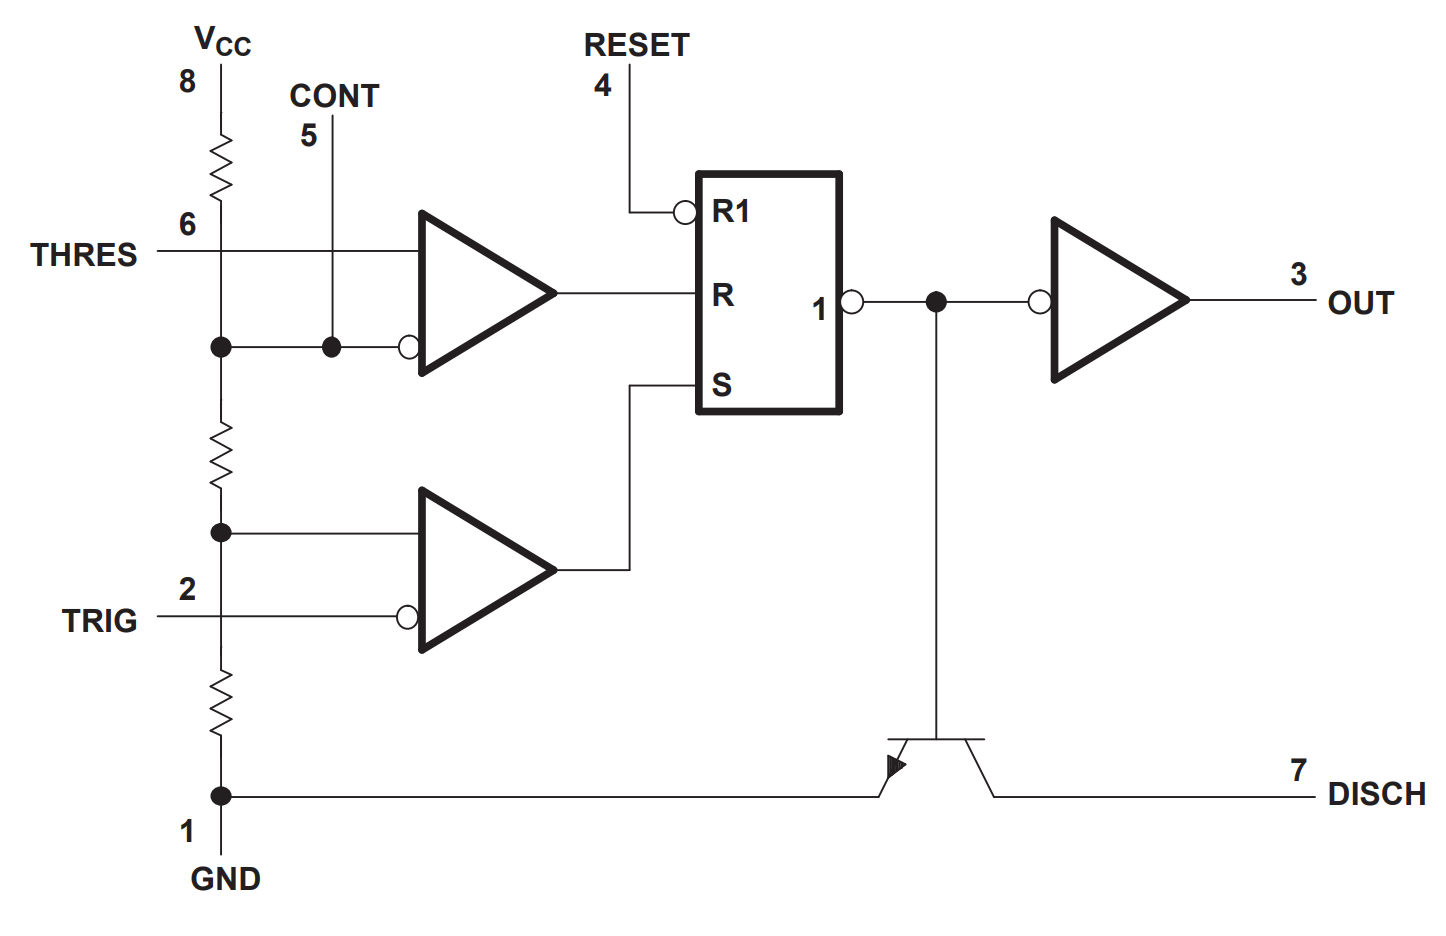
\includegraphics[width=0.45\textwidth]{../截图/NE555内部结构}
				\caption{NE555内部结构框图}
				\label{fig:NE555内部结构}
			\end{figure}
			NE555有三种常见的工作模式：单稳态、多稳态和无稳态模式。
			
			在本次仿真实验中需要使用NE555搭建脉冲发生电路，因此使用的是其多稳态工作模式，其电路连接方式如图\ref{fig:脉冲发生电路}：
			\begin{figure}[H]
				\centering
				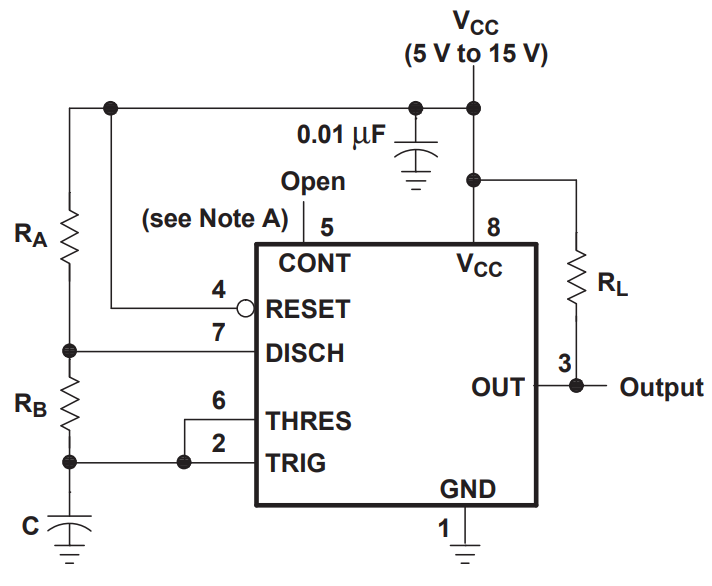
\includegraphics[width=0.45\textwidth]{../截图/脉冲发生电路}
				\caption{NE555脉冲发生电路}
				\label{fig:脉冲发生电路}
			\end{figure}
			此电路可以生成稳定的PWM方波信号，以下为该信号频率$f$和占空比$D\%$计算公式：		
			\begin{gather}
				f=\frac{1.44}{(R_A+2R_B)C}
				\label{con:NE555频率计算公式}
				\\
				D \% =\frac{R_A+R_B}{R_A+2R_B} \times 100 \%
				\label{con:NE555占空比计算公式}
			\end{gather}
		\subsection{可编程定时/计数器8253}
			8253是Intel公司生产的三通道16b的可编程定时/计数器，是具有24根引脚的双列直插式器件。\cite{book}
			
			其内部结构框图\cite{8253datasheet}如图\ref{fig:8253内部框图}所示，主要包括三个计数器、一个控制寄存器以及数据总线缓冲器和读写逻辑电路。
			\begin{figure}[H]
				\centering
				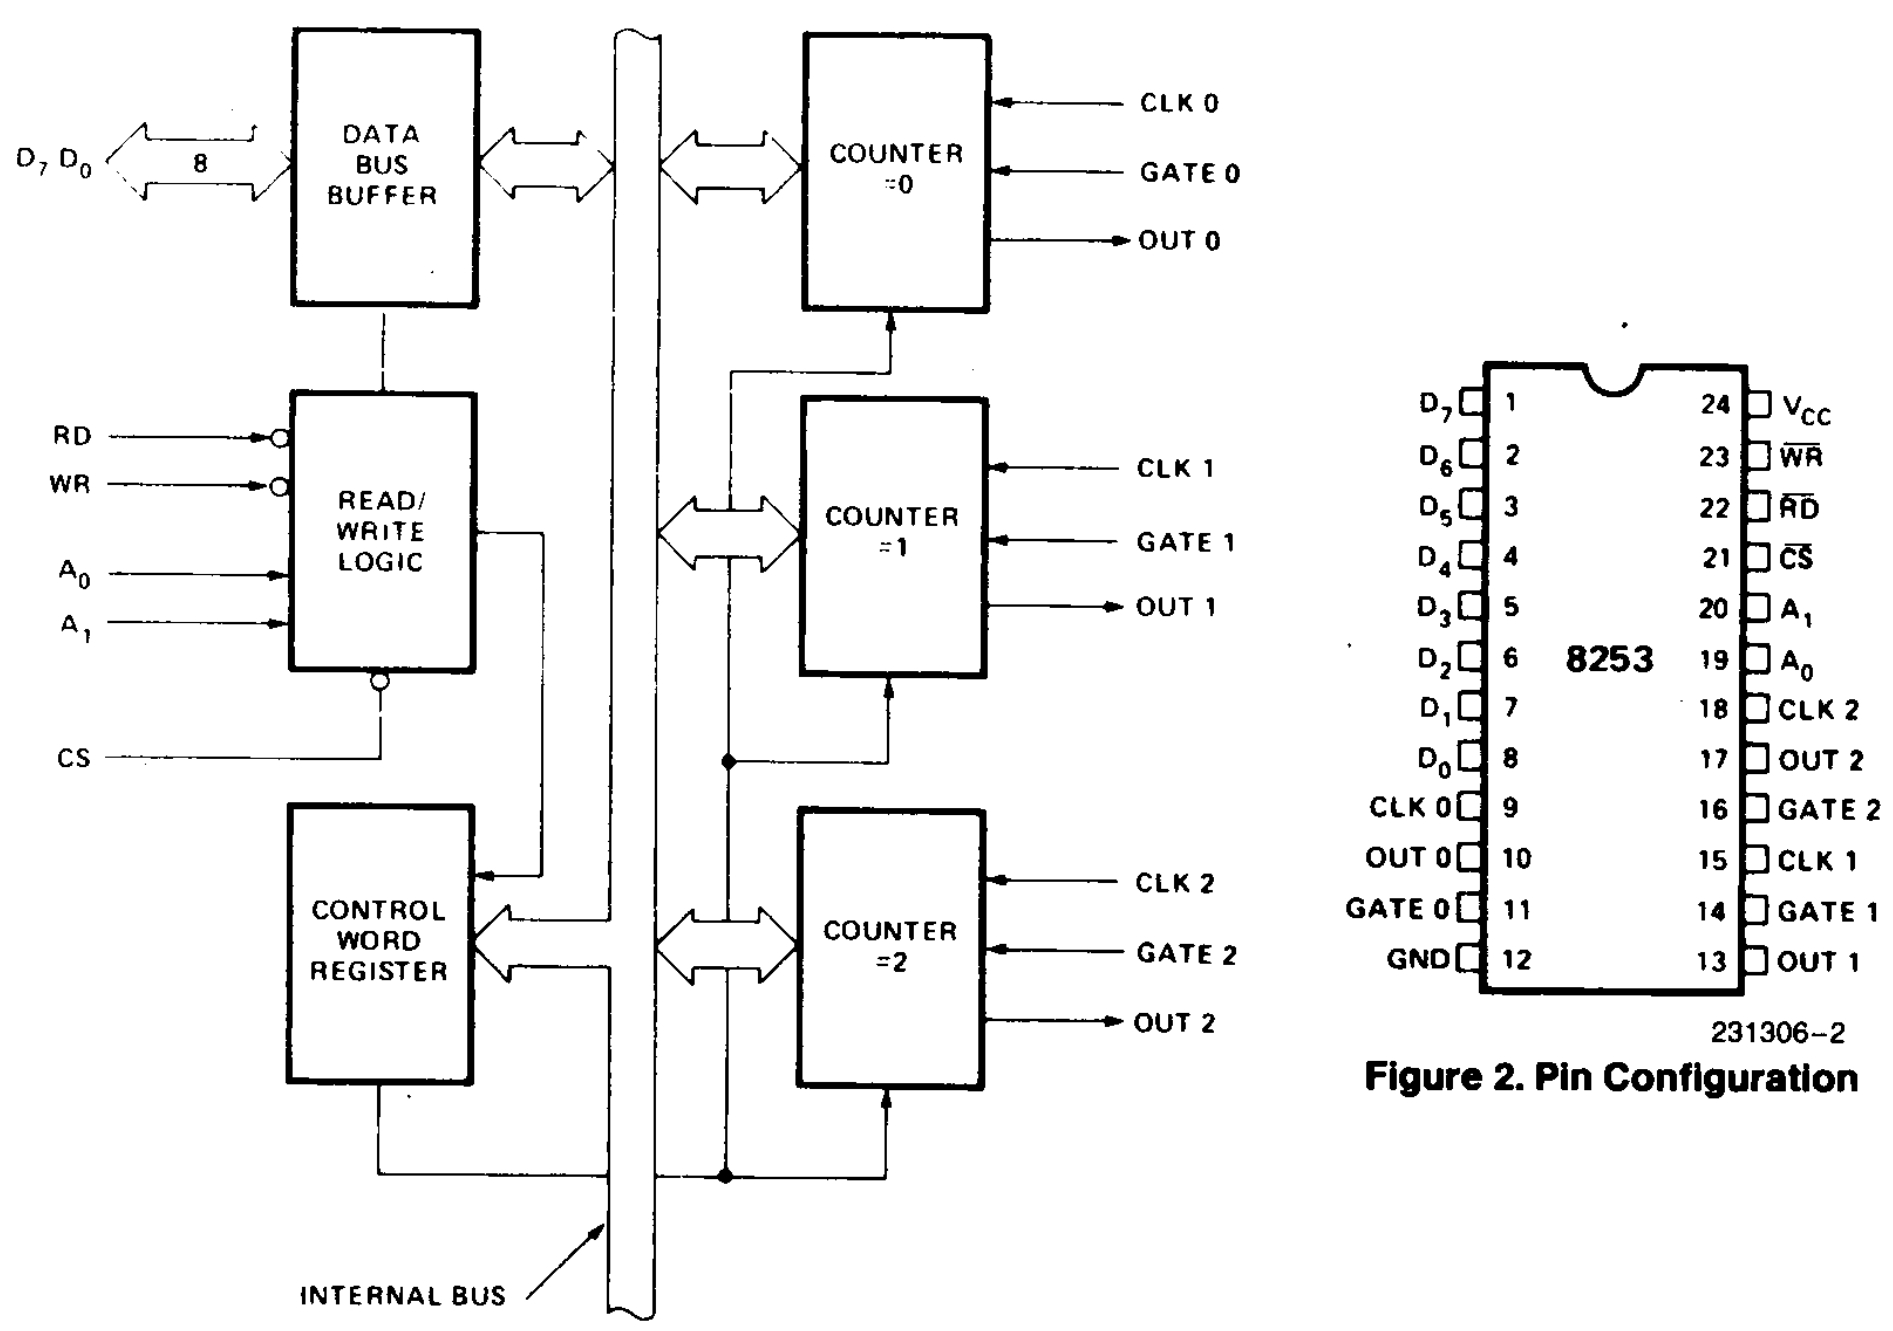
\includegraphics[width=0.45\textwidth]{../截图/8253内部框图}
				\caption{8253内部结构框图}
				\label{fig:8253内部框图}
			\end{figure}
			其控制字格式和初始化编程顺序如图\ref{fig:8253初始化相关参数}所示。
			\begin{figure}[h]
				\begin{subfigure}{0.5\linewidth}
					\centering
					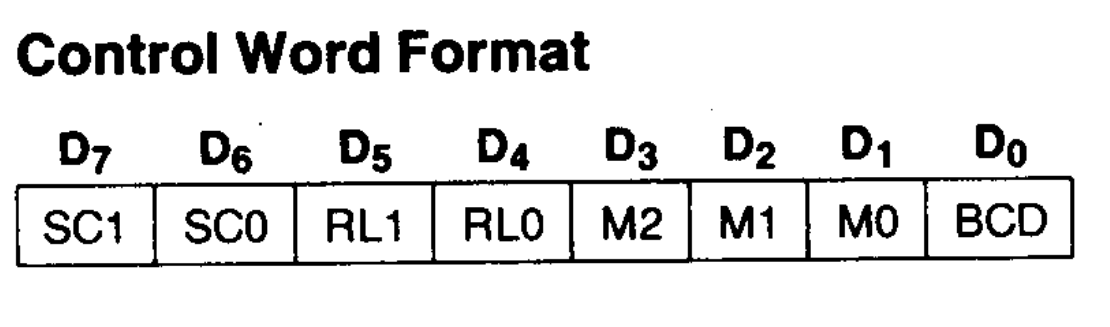
\includegraphics[width=0.9\linewidth]{../截图/8253控制字格式}
					\caption{8253控制字格式}
				\end{subfigure}
				\begin{subfigure}{0.5\linewidth}
					\centering
					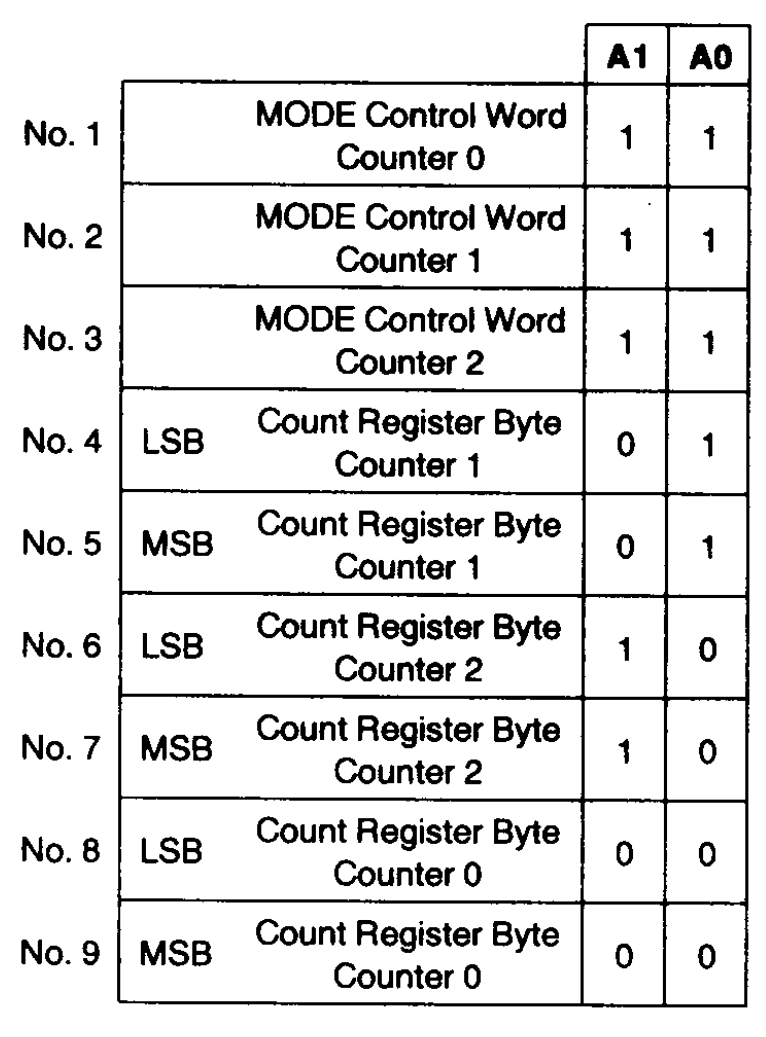
\includegraphics[width=0.45\linewidth]{../截图/8253初始化编程顺序}
					\caption{8253初始化编程顺序}
					\label{fig:8253初始化编程顺序}
				\end{subfigure}
				\caption{8253初始化}
				\label{fig:8253初始化相关参数}
			\end{figure}
			本次仿真采用两个分频器串联进行，因此仅使用计数器0和计数器1，选择两者的工作方式均为方波发生器，只读写计数器低八位。
			
			需要对\ref{fig:8253初始化编程顺序}中的初始化顺序进行删减，删去初始化计数器2的流程和对计数器高八位（MSB）的写入流程。
		\subsection{可编程中断控制器8259A}
			8259A是Intel公司生产的专为8086/8088CPU配套的可编程中断控制器，用于对8086/8088系统中的可屏蔽中断进行管理。8259A可对8个中断源实现优先级控制。8259A可以根据不同的中断源向CPU提供不同的中断类型码，还可根据需要对中断源进行中断屏蔽。8259A有多种工作方式，可以通过编程来选择，以适应不同的应用场合。\cite{book}
			
			其内部结构框图\cite{8259Adatasheet}如图\ref{fig:8259A内部框图}所示。
			\begin{figure}[H]
				\centering
				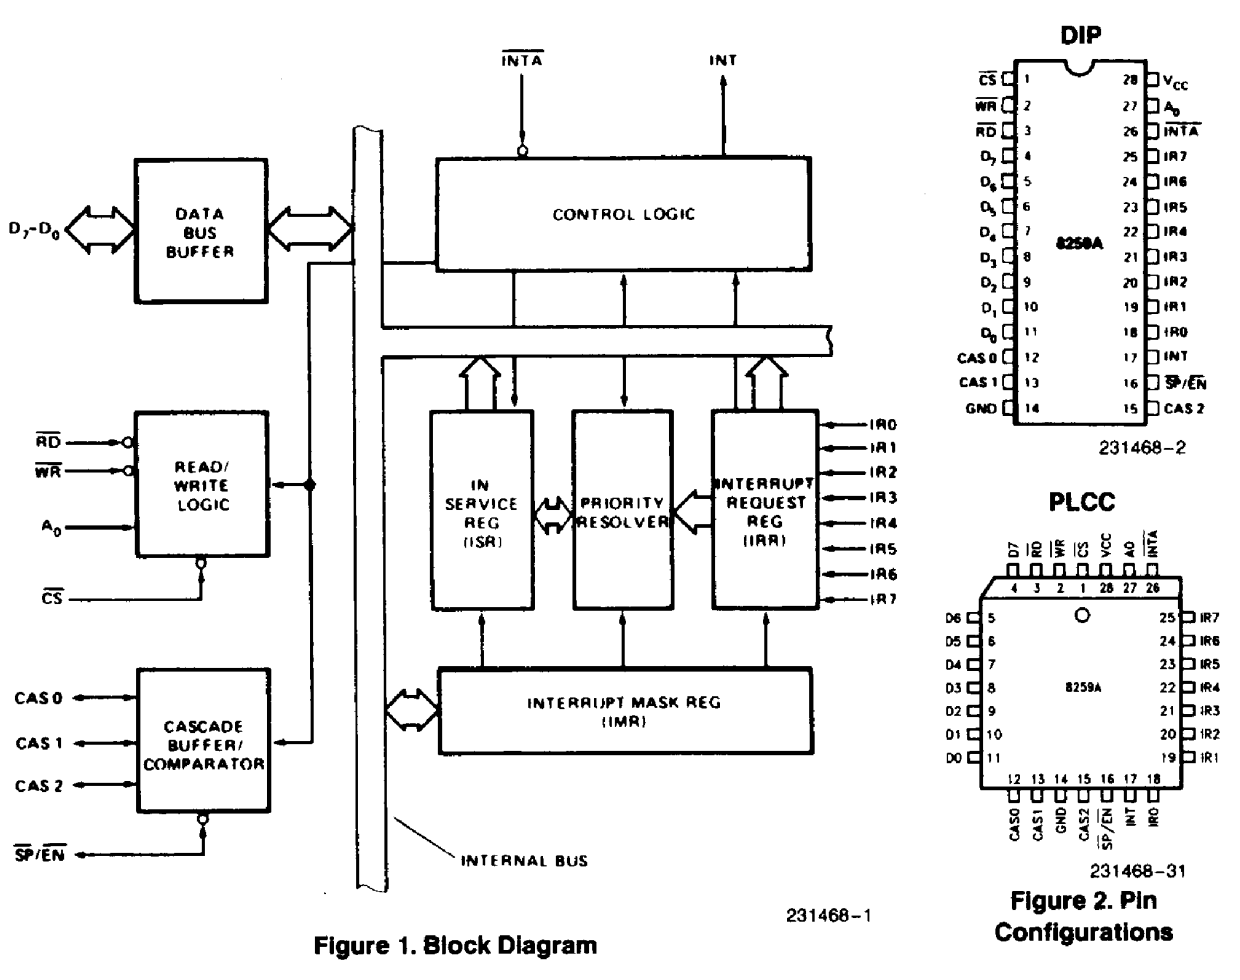
\includegraphics[width=0.45\textwidth]{../截图/8259A内部框图}
				\caption{8259A内部结构框图}
				\label{fig:8259A内部框图}
			\end{figure}
			其初始化涉及四条初始化命令字（ICW）和三条操作命令字（OCW），由于篇幅限制将不在此列出具体指令的含义。
			
			其控制字格式和初始化编程顺序如图\ref{fig:8259A初始化编程顺序}所示。
			\begin{figure}[h]
				\centering
				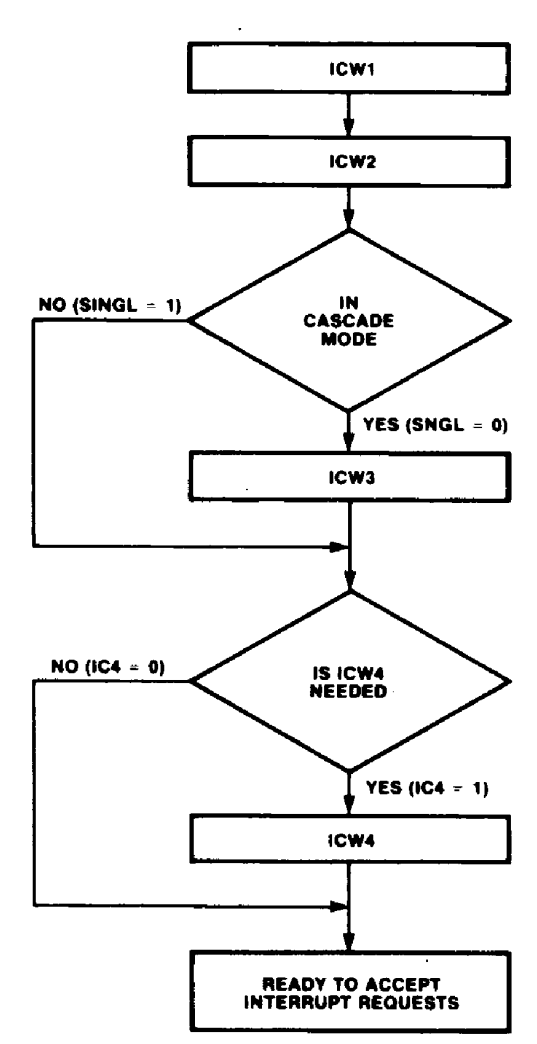
\includegraphics[width=0.3\textwidth]{../截图/8259A初始化编程顺序}
				\caption{8259A初始化编程顺序}
				\label{fig:8259A初始化编程顺序}
			\end{figure}
			本次仿真只有一个中断源。因此，不使用初始化命令字ICW3和操作命令字OCW1、OCW3。
			
			对于8086芯片，中断需要向内存中的中断向量表中指明中断服务函数的代码段段基地址和子程序偏移地址，故在初始化8259A后应当初始化向量表。
		\subsection{可编程并行接口8255}
			Intel 8255A是一个通用目的可编程I/O设备，设计用于与Intel微处理器一起使用。它拥有24个I/O引脚，这些引脚可以单独编程为两组各12个引脚，并在三种主要操作模式下使用。在第一种模式（模式0）中，每组12个I/O引脚可以编程为每组4个引脚作为输入或输出。在第二种模式（模式1）中，每组可以编程为具有8条输入或输出线。在剩余的4个引脚中，有3个用于握手和中断控制信号。第三种操作模式（模式2）是双向总线模式，它使用8条线作为双向总线，并借用另一组的1条线用于握手，共5条线。\cite{8255datasheet}
			
			其内部结构框图\cite{8255datasheet}如图\ref{fig:8255内部框图}所示。
			\begin{figure}[H]
				\centering
				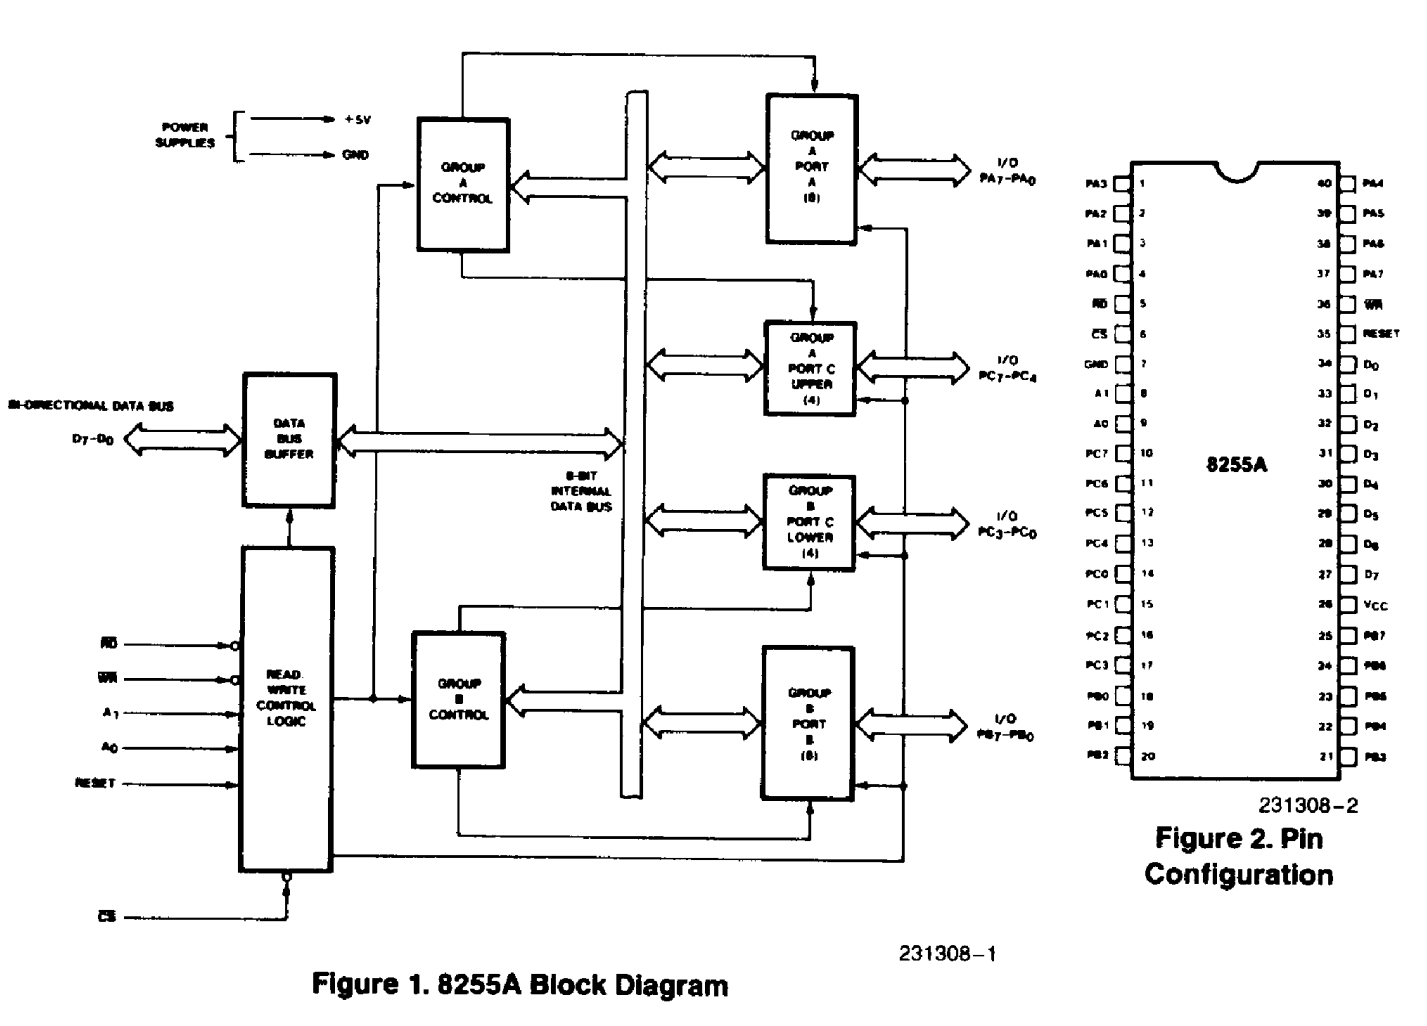
\includegraphics[width=0.45\textwidth]{../截图/8255内部框图}
				\caption{8255内部结构框图}
				\label{fig:8255内部框图}
			\end{figure}
			本次仿真使用8255的并行口均在模式0下工作，其中，PA口作为输出，PB口作为输入，根据8255芯片控制字规则可知道对应的控制字应为10000010B=82H。
		\subsection{LED显示芯片MAX7219}
			MAX7219/MAX7221为紧凑的串行输入/输出共阴极显示驱动器，用于连接微处理器(µP)与8位7段LED数码管显示器、条形图显示器或64个独立的LED。器件内置BCD B码译码器、多路复用扫描电路、段和位驱动器以及存储每位数字的8x8静态RAM。只需一个外部电阻即可设置所有LED的段电流。MAX7221兼容于SPI™、QSPI™以及MICROWIRE™接口，段驱动器带有摆率限制，以降低EMI。\cite{MAX7219datasheet}
			\begin{figure}[H]
				\begin{subfigure}{0.5\linewidth}
					\centering
					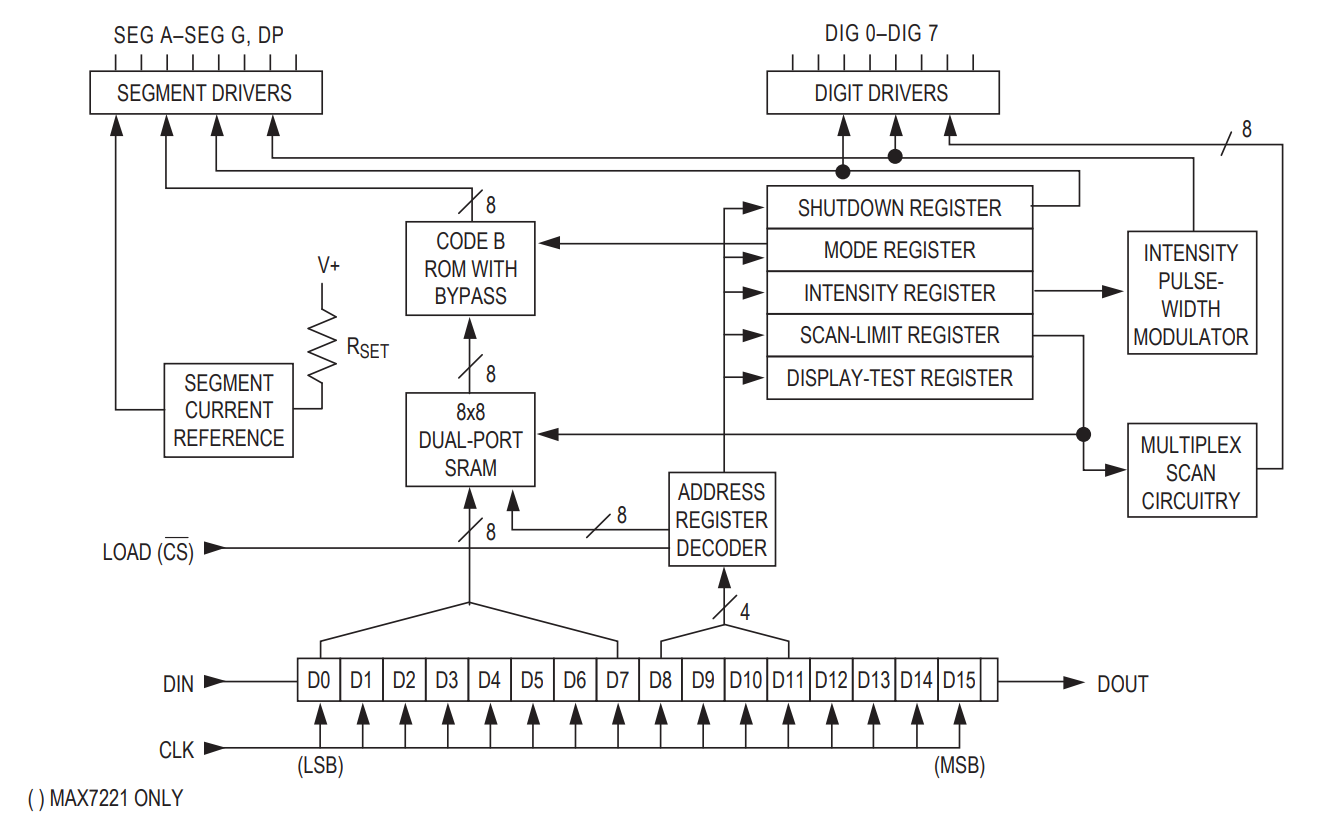
\includegraphics[width=0.9\linewidth]{../截图/MAX7219内部框图}
					\caption{MAX7219内部结构框图}
					\label{fig:MAX7219内部结构框图}
				\end{subfigure}
				\begin{subfigure}{0.5\linewidth}
					\centering
					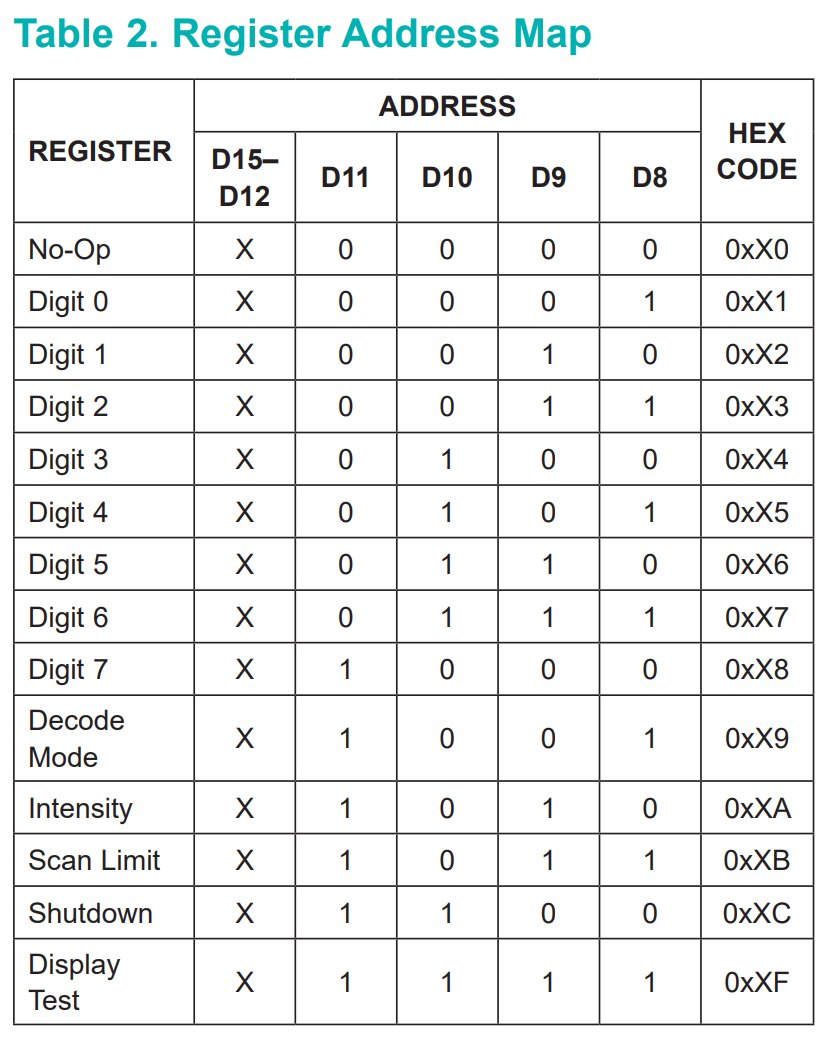
\includegraphics[width=0.45\linewidth]{../截图/MAX7219寄存器地址图}
					\caption{MAX7219寄存器地址图}
					\label{fig:MAX7219寄存器地址图}
				\end{subfigure}
				\caption{MAX7219芯片参数图}
				\label{fig:MAX7219芯片参数图}
			\end{figure}
			MAX7219内部结构框图如图\ref{fig:MAX7219内部结构框图}所示，其内部自带多路复用扫描电路（MULTIPLEX SCAN CIRCUITRY)，可以自动进行扫描显示，方便了点阵的显示。
			
			接口使用SPI时序，高八位地址，低八位数据的格式通信，其具体寄存器组如图\ref{fig:MAX7219寄存器地址图}所示，寄存器的使用将在软件编程初始化中体现。
		\subsection{移位寄存器74LS595}
			74LS595是串行输入并行输出的器件，可以串联使用，达到引脚拓展的目的。主要引用在数码管的驱动，点阵的驱动等需要多个引脚的地方。
			\begin{figure}[H]
				\centering
				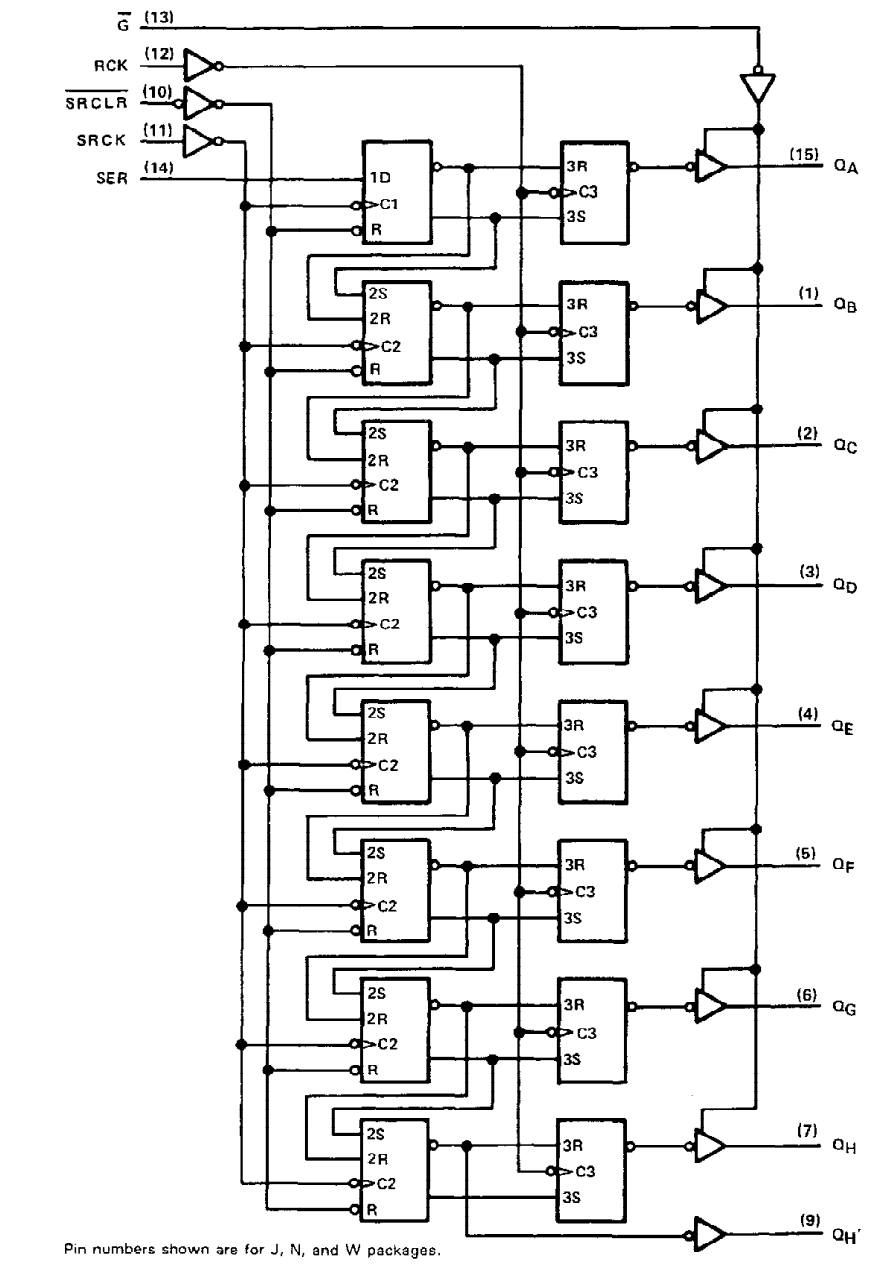
\includegraphics[width=0.25\textwidth]{../截图/74LS595内部框图}
				\caption{74LS595内部结构框图}
				\label{fig:74LS595内部框图}
			\end{figure}
			74LS595芯片内部结构如图\ref{fig:74LS595内部框图}所示\cite{74LS595datasheet}，其本质是八个主从D触发器串联，其八位输出每个分别与一个三态门串联。
			
			其中，输入时序与SPI时序类似，只是多了个SCK的输出使能引脚。可以参考软件SPI时序的写法结合可编程并行接口芯片8255的特点进行代码编写。
	\newpage
	\section{硬件设计}
		硬件整体设计分为如下四个部分：
		\begin{compactenum}
			\item 定时器中断部分硬件设计；
			\item 点阵显示部分硬件设计；
			\item 数码管显示部分硬件设计；
			\item 按键输入部分硬件设计。
		\end{compactenum}
		
		根据上述任务简述，绘制出硬件电路总图，如图\ref{fig:硬件设计总图}。
		\begin{figure}[H]
			\centering
			\includegraphics[width=0.5\textwidth]{../截图/硬件设计总图}
			\caption{硬件设计总图}
			\label{fig:硬件设计总图}
		\end{figure}
		如下，将对每个部分的设计一一作出介绍。
		\subsection{定时器中断部分}
			定时器部分主要采用脉冲发生器NE555芯片、可编程定时/计数器芯片8253和可编程中断控制器芯片8259A完成，其原理图如图\ref{fig:定时器中断部分硬件设计}所示：
			\begin{figure}[H]
				\centering
				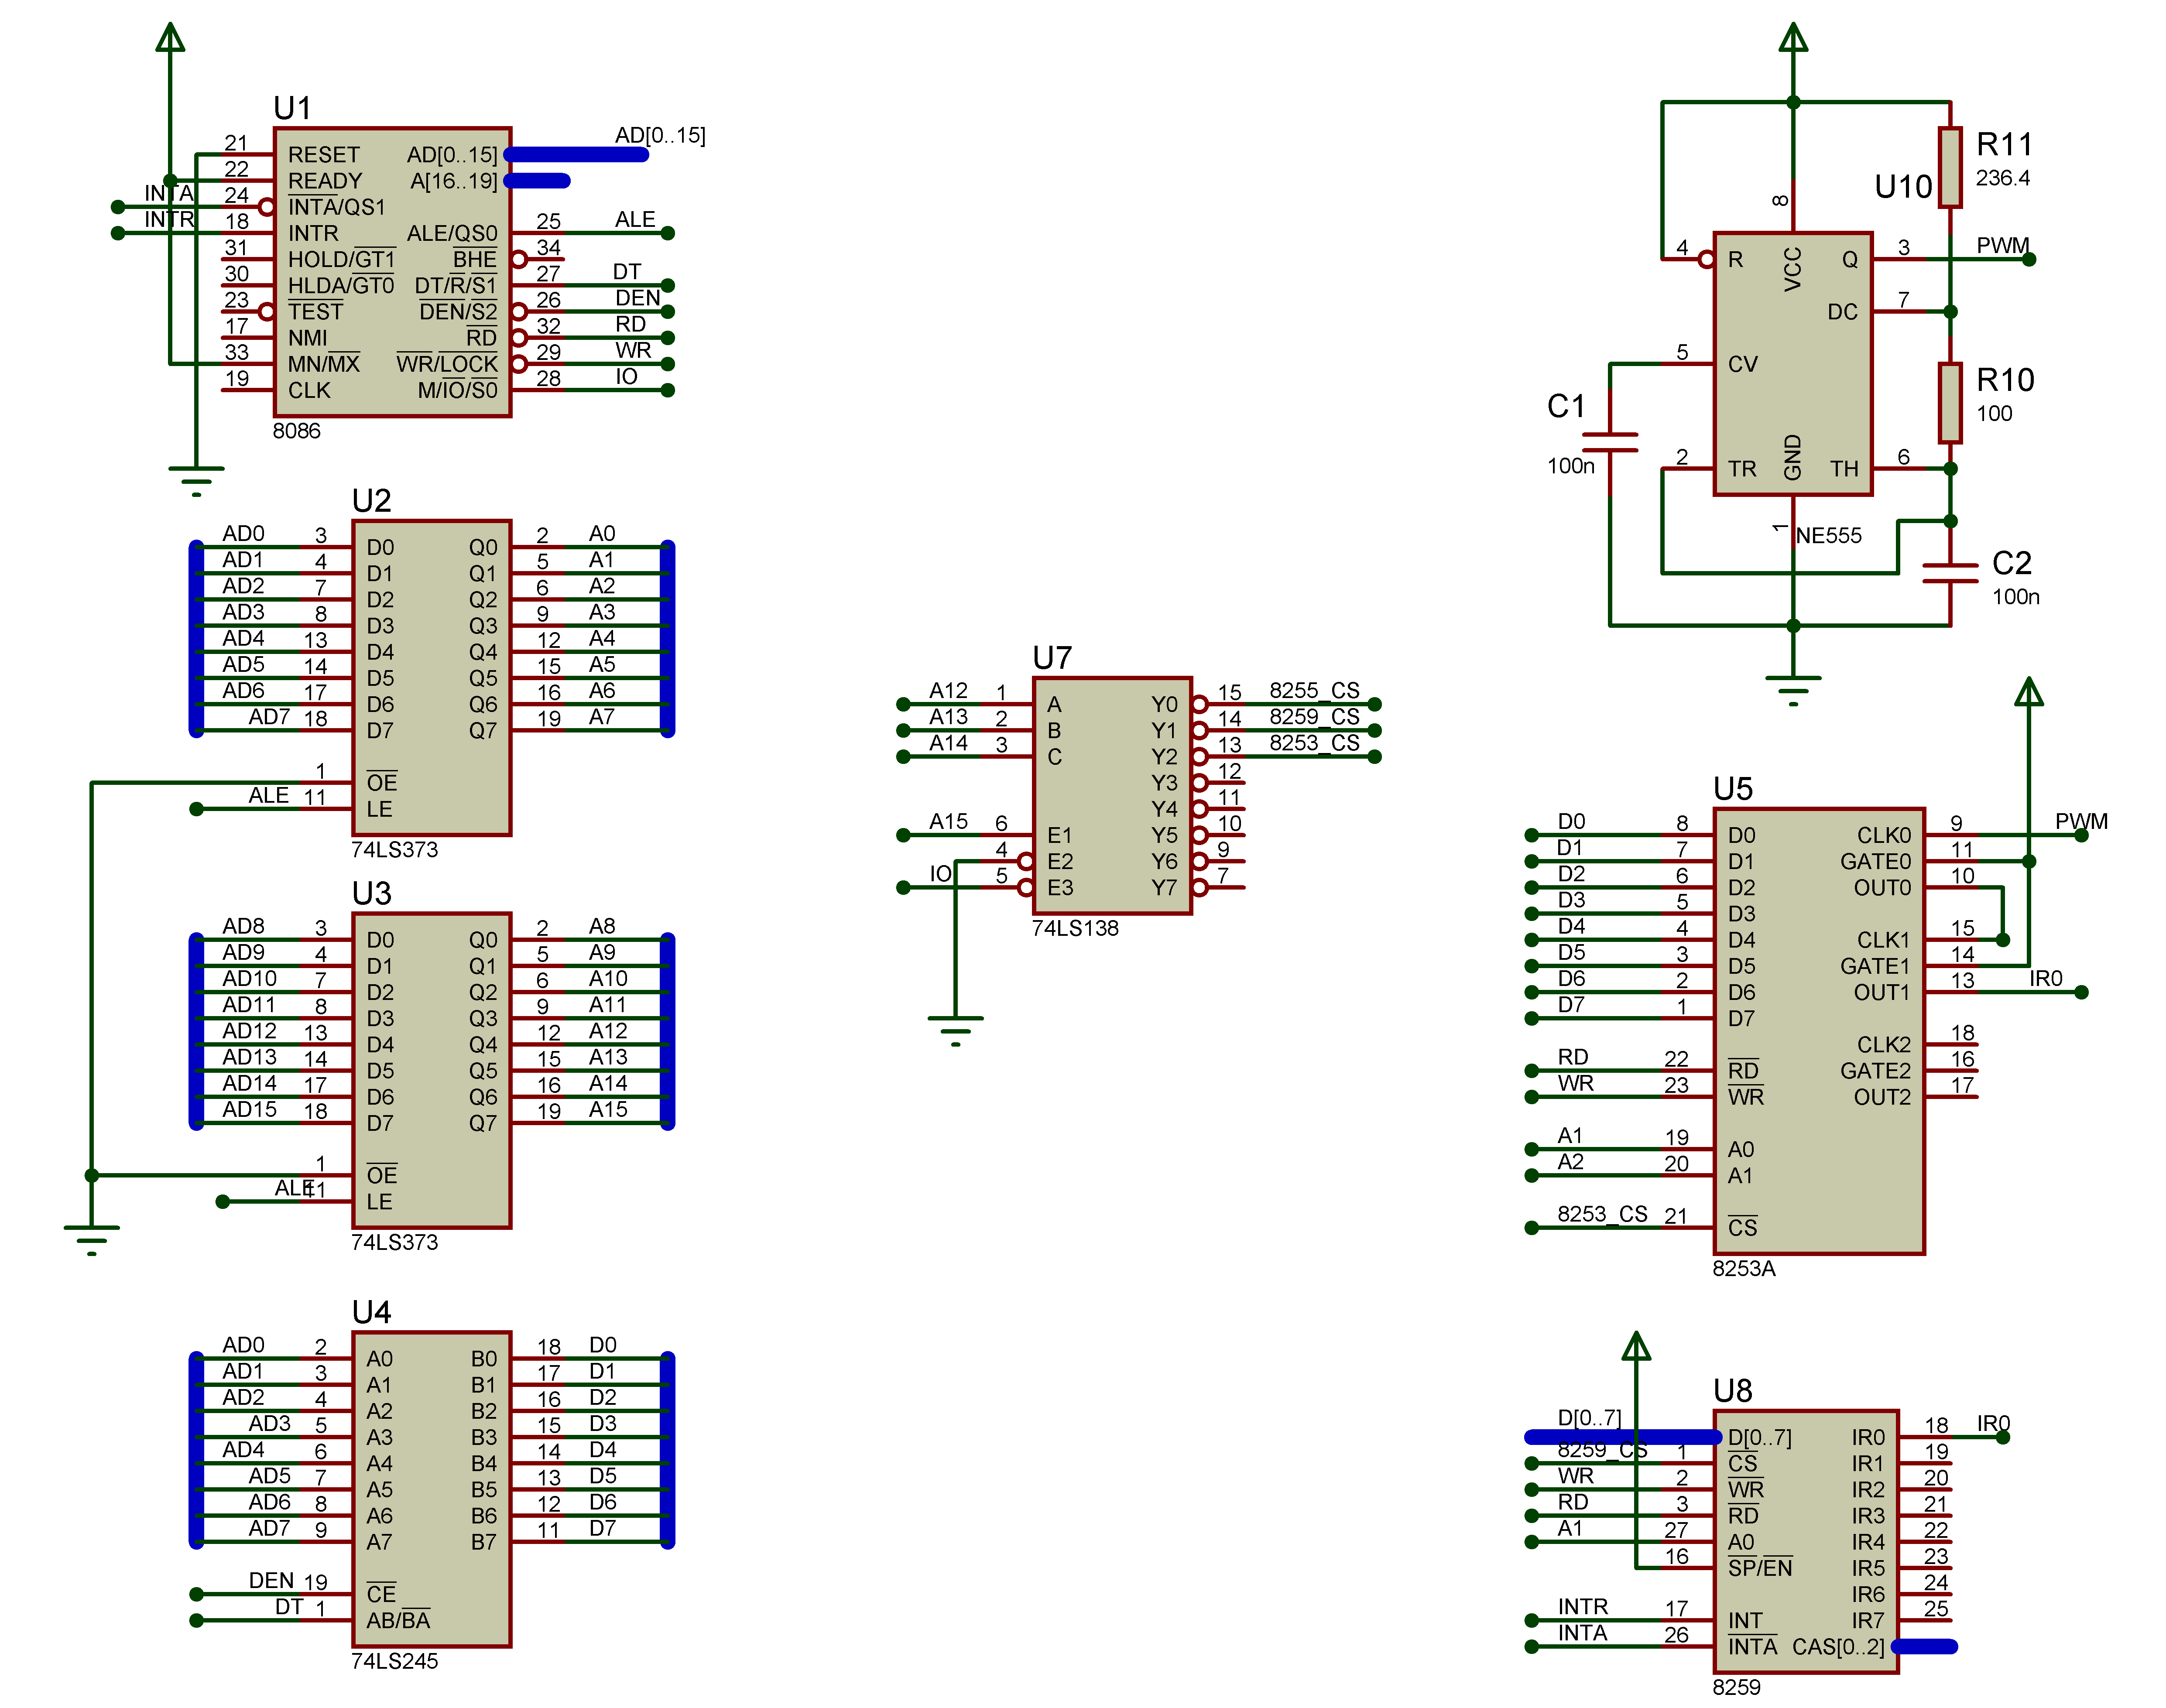
\includegraphics[width=0.5\textwidth]{../截图/定时器中断部分硬件设计}
				\caption{定时器中断部分原理图}
				\label{fig:定时器中断部分硬件设计}
			\end{figure}
			
			电路采用NE555芯片作为时基信号发生器，生成32768Hz的频率，根据公式\ref{con:NE555频率计算公式}，可反推出对应电阻电容计算公式，因为此处信号只对周期时间有所要求，对占空比无要求，故可采用值较多，此处选择了$R_A=236.4 \Omega$、$R_B=100 \Omega$、$C=100nF$的组合。
			
			生成的信号将输入8253的计数器0，经过计数器0的分频后再次进入计数器1。通过两次的计时器分频可以将输入32768Hz，十五倍分频得到1Hz的标准秒频率。以此达到每一秒触发一次定时器中断的目的。
			
			其中，8253的$A0$和$A1$引脚分别与8086芯片的$AD1$和$AD2$相通，片选引脚$\overline{CS}$与译码器芯片的$\overline{Y2}$，故可以推得对应其映射地址，如表\ref{tab:8253芯片的外设地址}所示。
			\begin{table}[h!]
				\centering
				\caption{8253芯片的外设地址}
				\begin{tabular}{c|c|c}
					端口 & 二进制地址 & 采用值\\
					\hline\hline
					计数器0 & 1011 xxxx xxxx x00xB &A000H\\
					计数器1 & 1011 xxxx xxxx x01xB &A002H\\
					计数器2 & 1011 xxxx xxxx x10xB &A004H\\
					控制字  & 1011 xxxx xxxx x11xB &A006H\\
				\end{tabular}
				\label{tab:8253芯片的外设地址}
			\end{table}
			
			最后将8253的输出信号与8259A芯片的IR0相连，以此将中断信号传入中断控制器芯片，中断控制器的$INT$引脚与8086的$\overline{INTA}/QS1$引脚、$\overline{INTR}$引脚8086的$INTR$引脚相连，达到将可屏蔽中断信号传入CPU中的目的。从而达到引发中断。
			
			其中，8259A的$A0$引脚与8086芯片的$AD1$相通，片选引脚$\overline{CS}$与译码器芯片的$\overline{Y1}$，故可以推得对应其映射地址，如表\ref{tab:8259A芯片的外设地址}所示。
			\begin{table}[h!]
				\centering
				\caption{8259A芯片的外设地址}
				\begin{tabular}{c|c|c}
					控制字 & 二进制地址 & 采用值\\
					\hline\hline
					ICW1 & 1010 xxxx xxxx xx0xB &9000H\\
					ICW2 & 1010 xxxx xxxx xx1xB &9002H\\
					ICW3 & 1010 xxxx xxxx xx1xB &9002H\\
					ICW4 & 1010 xxxx xxxx xx1xB &9002H\\
					\hline
					OCW1 & 1010 xxxx xxxx xx1xB &9002H\\
					OCW2 & 1010 xxxx xxxx xx0xB &9000H\\
					OCW3 & 1010 xxxx xxxx xx0xB &9000H\\
				\end{tabular}
				\label{tab:8259A芯片的外设地址}
			\end{table}
			
			以上，经过信号的发生，处理，最终以中断信号的形式输入到8086CPU中完成定时器中断的信号逻辑。
		\subsection{点阵显示部分}
			点阵显示部分采用LED显示芯片MAX7219驱动，8255作为预驱，其原理图如图\ref{fig:点阵显示部分硬件设计}所示。
			\begin{figure}[h]
				\centering
				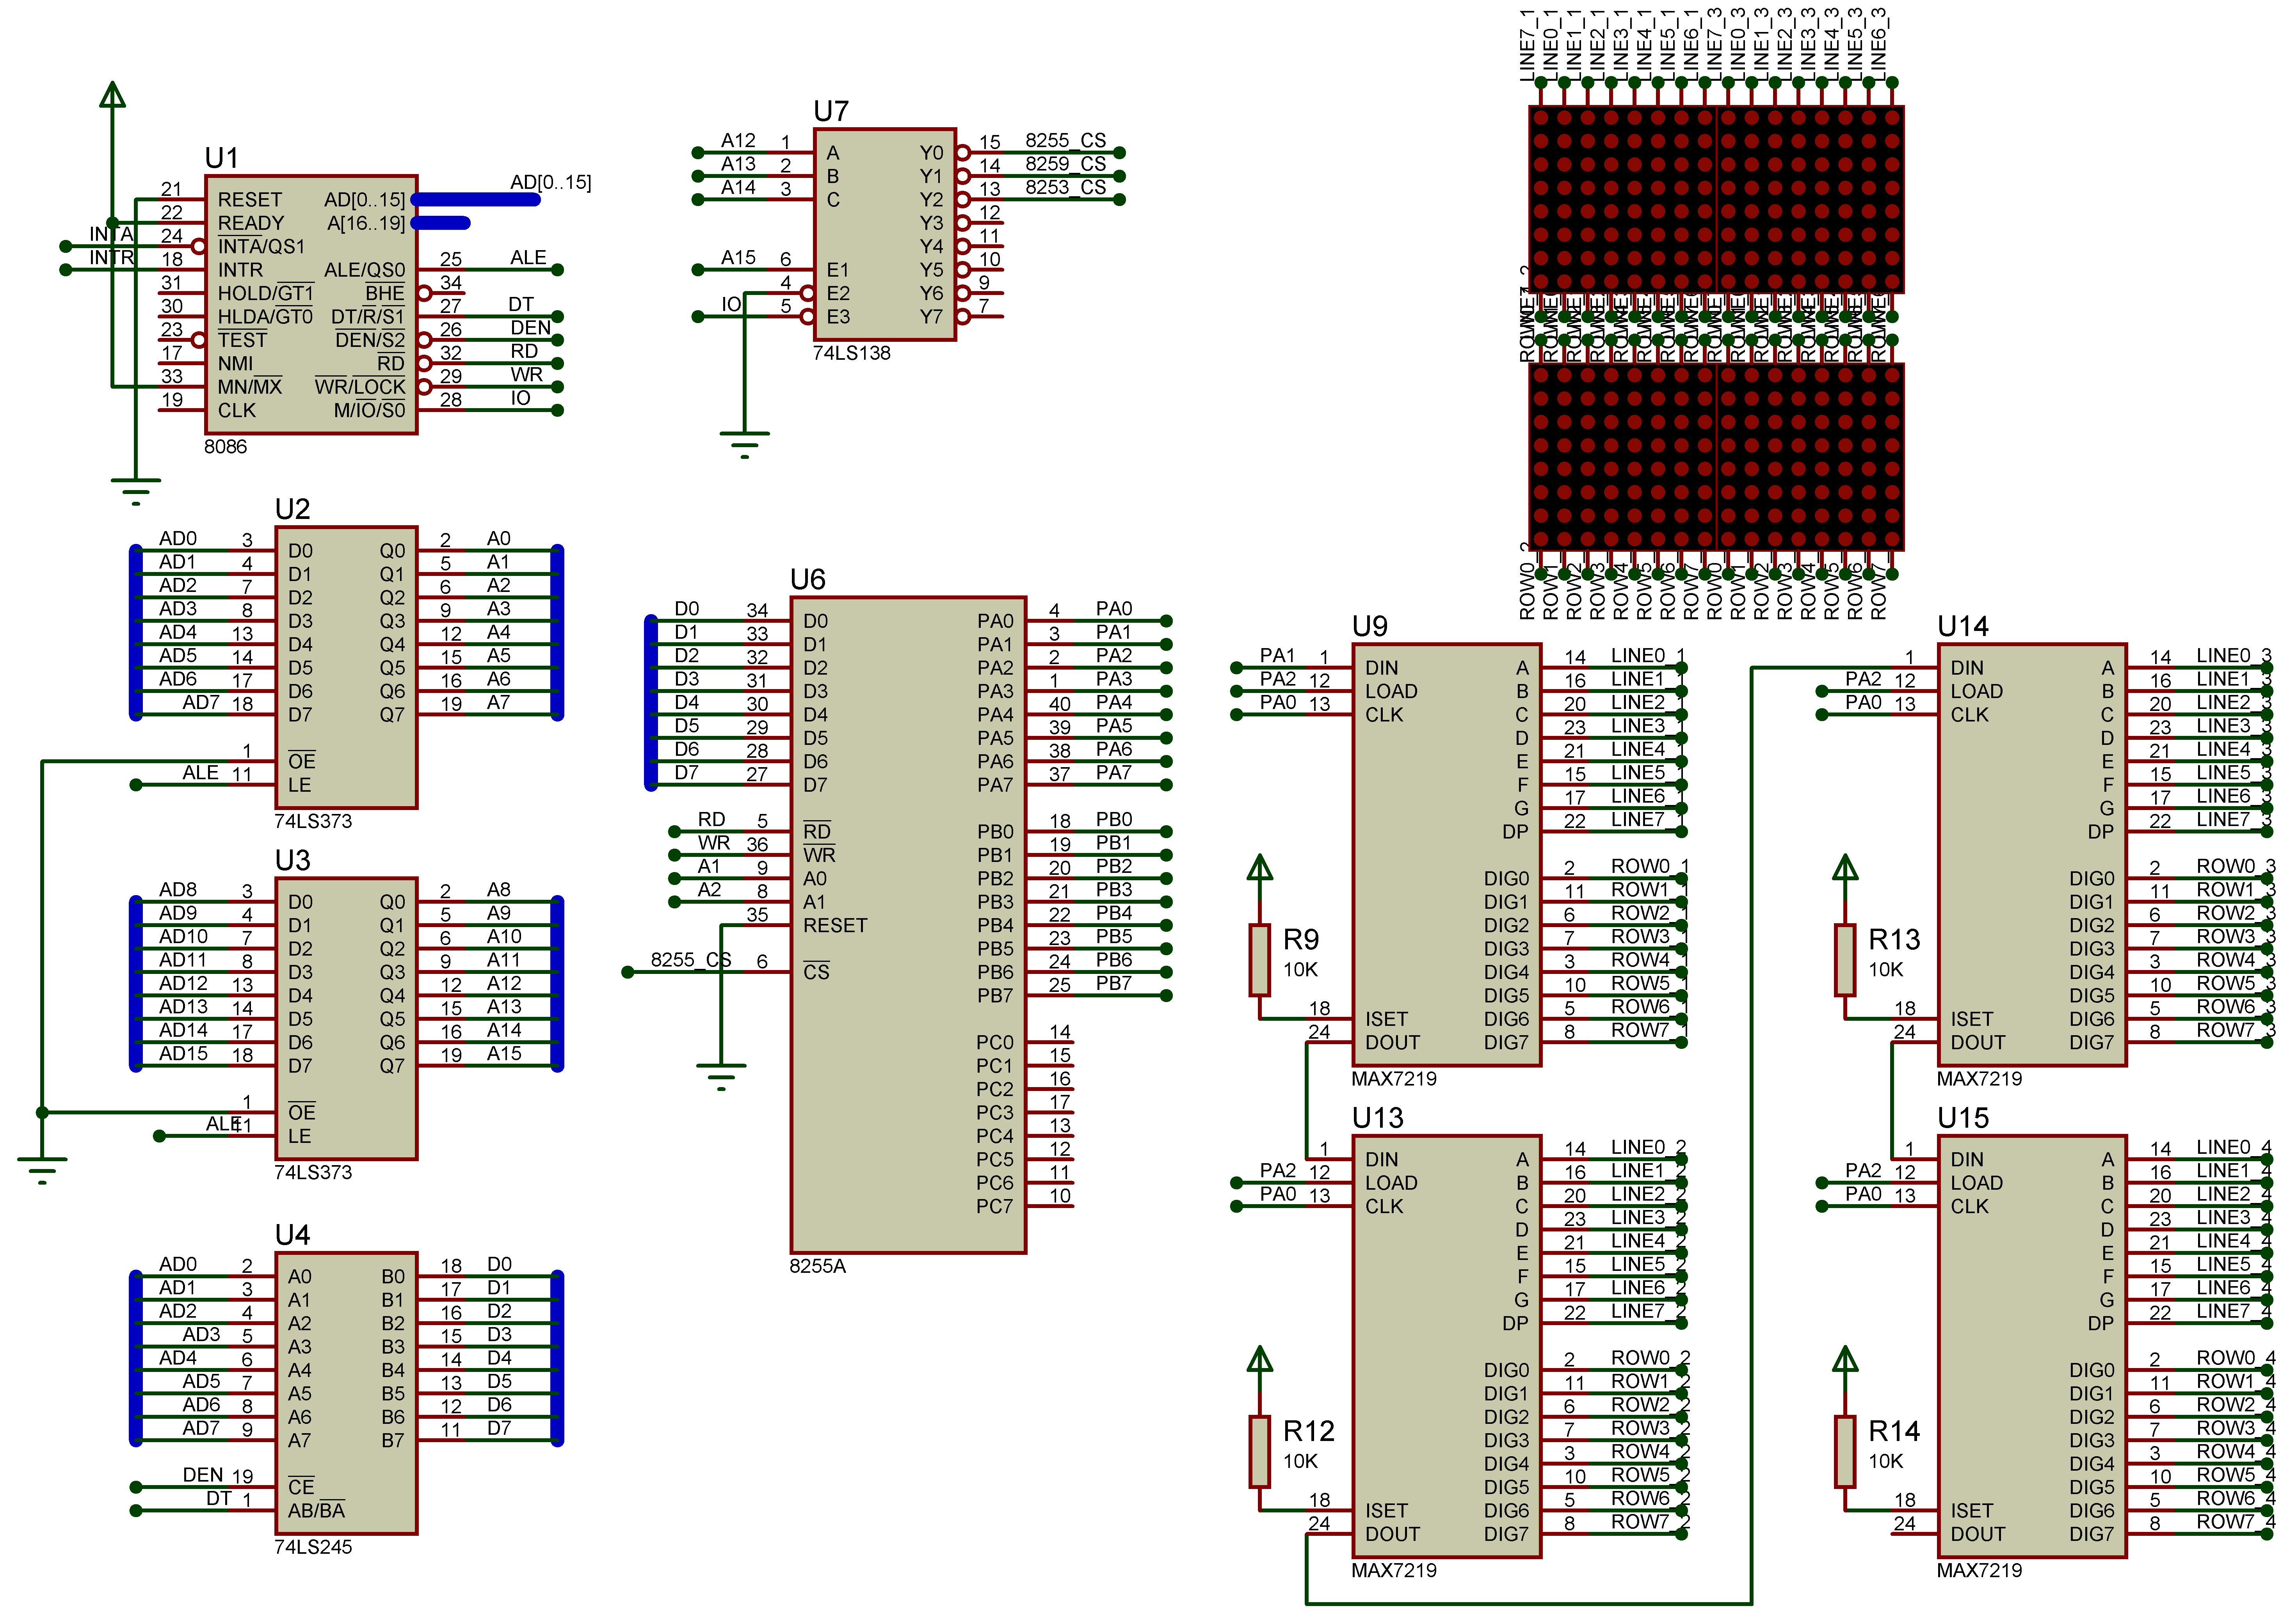
\includegraphics[width=0.5\textwidth]{../截图/点阵显示部分硬件设计}
				\caption{点阵显示部分原理图}
				\label{fig:点阵显示部分硬件设计}
			\end{figure}
			
			该部分，信号从8086输出后，经过8255的PA并行接口的引脚PA0、PA1、PA2三根信号线输出给MAX7129，MAX7219接收端从图\ref{fig:MAX7219内部结构框图}中可以看出是一个16比特的移位寄存器，从$Din$引脚输入，至$Dout$引脚输出，单独芯片完成16位数据收发
			
			此处，特意设置$CLK$引脚连接PA0，$Din$引脚连接PA1。如此可以实现，当输入数据的一刻，时钟线是低电平，下一个时刻通过$INC$将时钟拉高，如此减少了代码量。
			
			需要注意的是MAX7219芯片$DIGx$引脚原本应连接共阴极数码管的共阴极$COM$端，在8x8的数码管中，则应连接行选线。以及本次仿真使用4个8*8点阵构成，所以需要级联四片MAX7219芯片以驱动，每两片芯片之间$Din$连下一级的$Dout$。
			
			其中，8253的$A0$和$A1$引脚分别与8086芯片的$AD1$和$AD2$相通，片选引脚$\overline{CS}$与译码器芯片的$\overline{Y0}$，故可以推得对应其映射地址，如表\ref{tab:8255芯片的外设地址}所示。
			\begin{table}[h!]
				\centering
				\caption{8255芯片的外设地址}
				\begin{tabular}{c|c|c}
					端口 & 二进制地址 & 采用值\\
					\hline\hline
					端口A   & 1000 xxxx xxxx x00xB &8000H\\
					端口B   & 1000 xxxx xxxx x01xB &8002H\\
					端口C   & 1000 xxxx xxxx x10xB &8004H\\
					控制字  & 1000 xxxx xxxx x11xB &8006H\\
				\end{tabular}
				\label{tab:8255芯片的外设地址}
			\end{table}
			以上实现了使用并口芯片8255对四个点阵的驱动。
		\subsection{数码管显示部分}
			数码管显示部分采用移位寄存器74LS595驱动，8255作为预驱，其原理图如图\ref{fig:数码管显示部分硬件设计}所示。
			\begin{figure}[H]
				\centering
				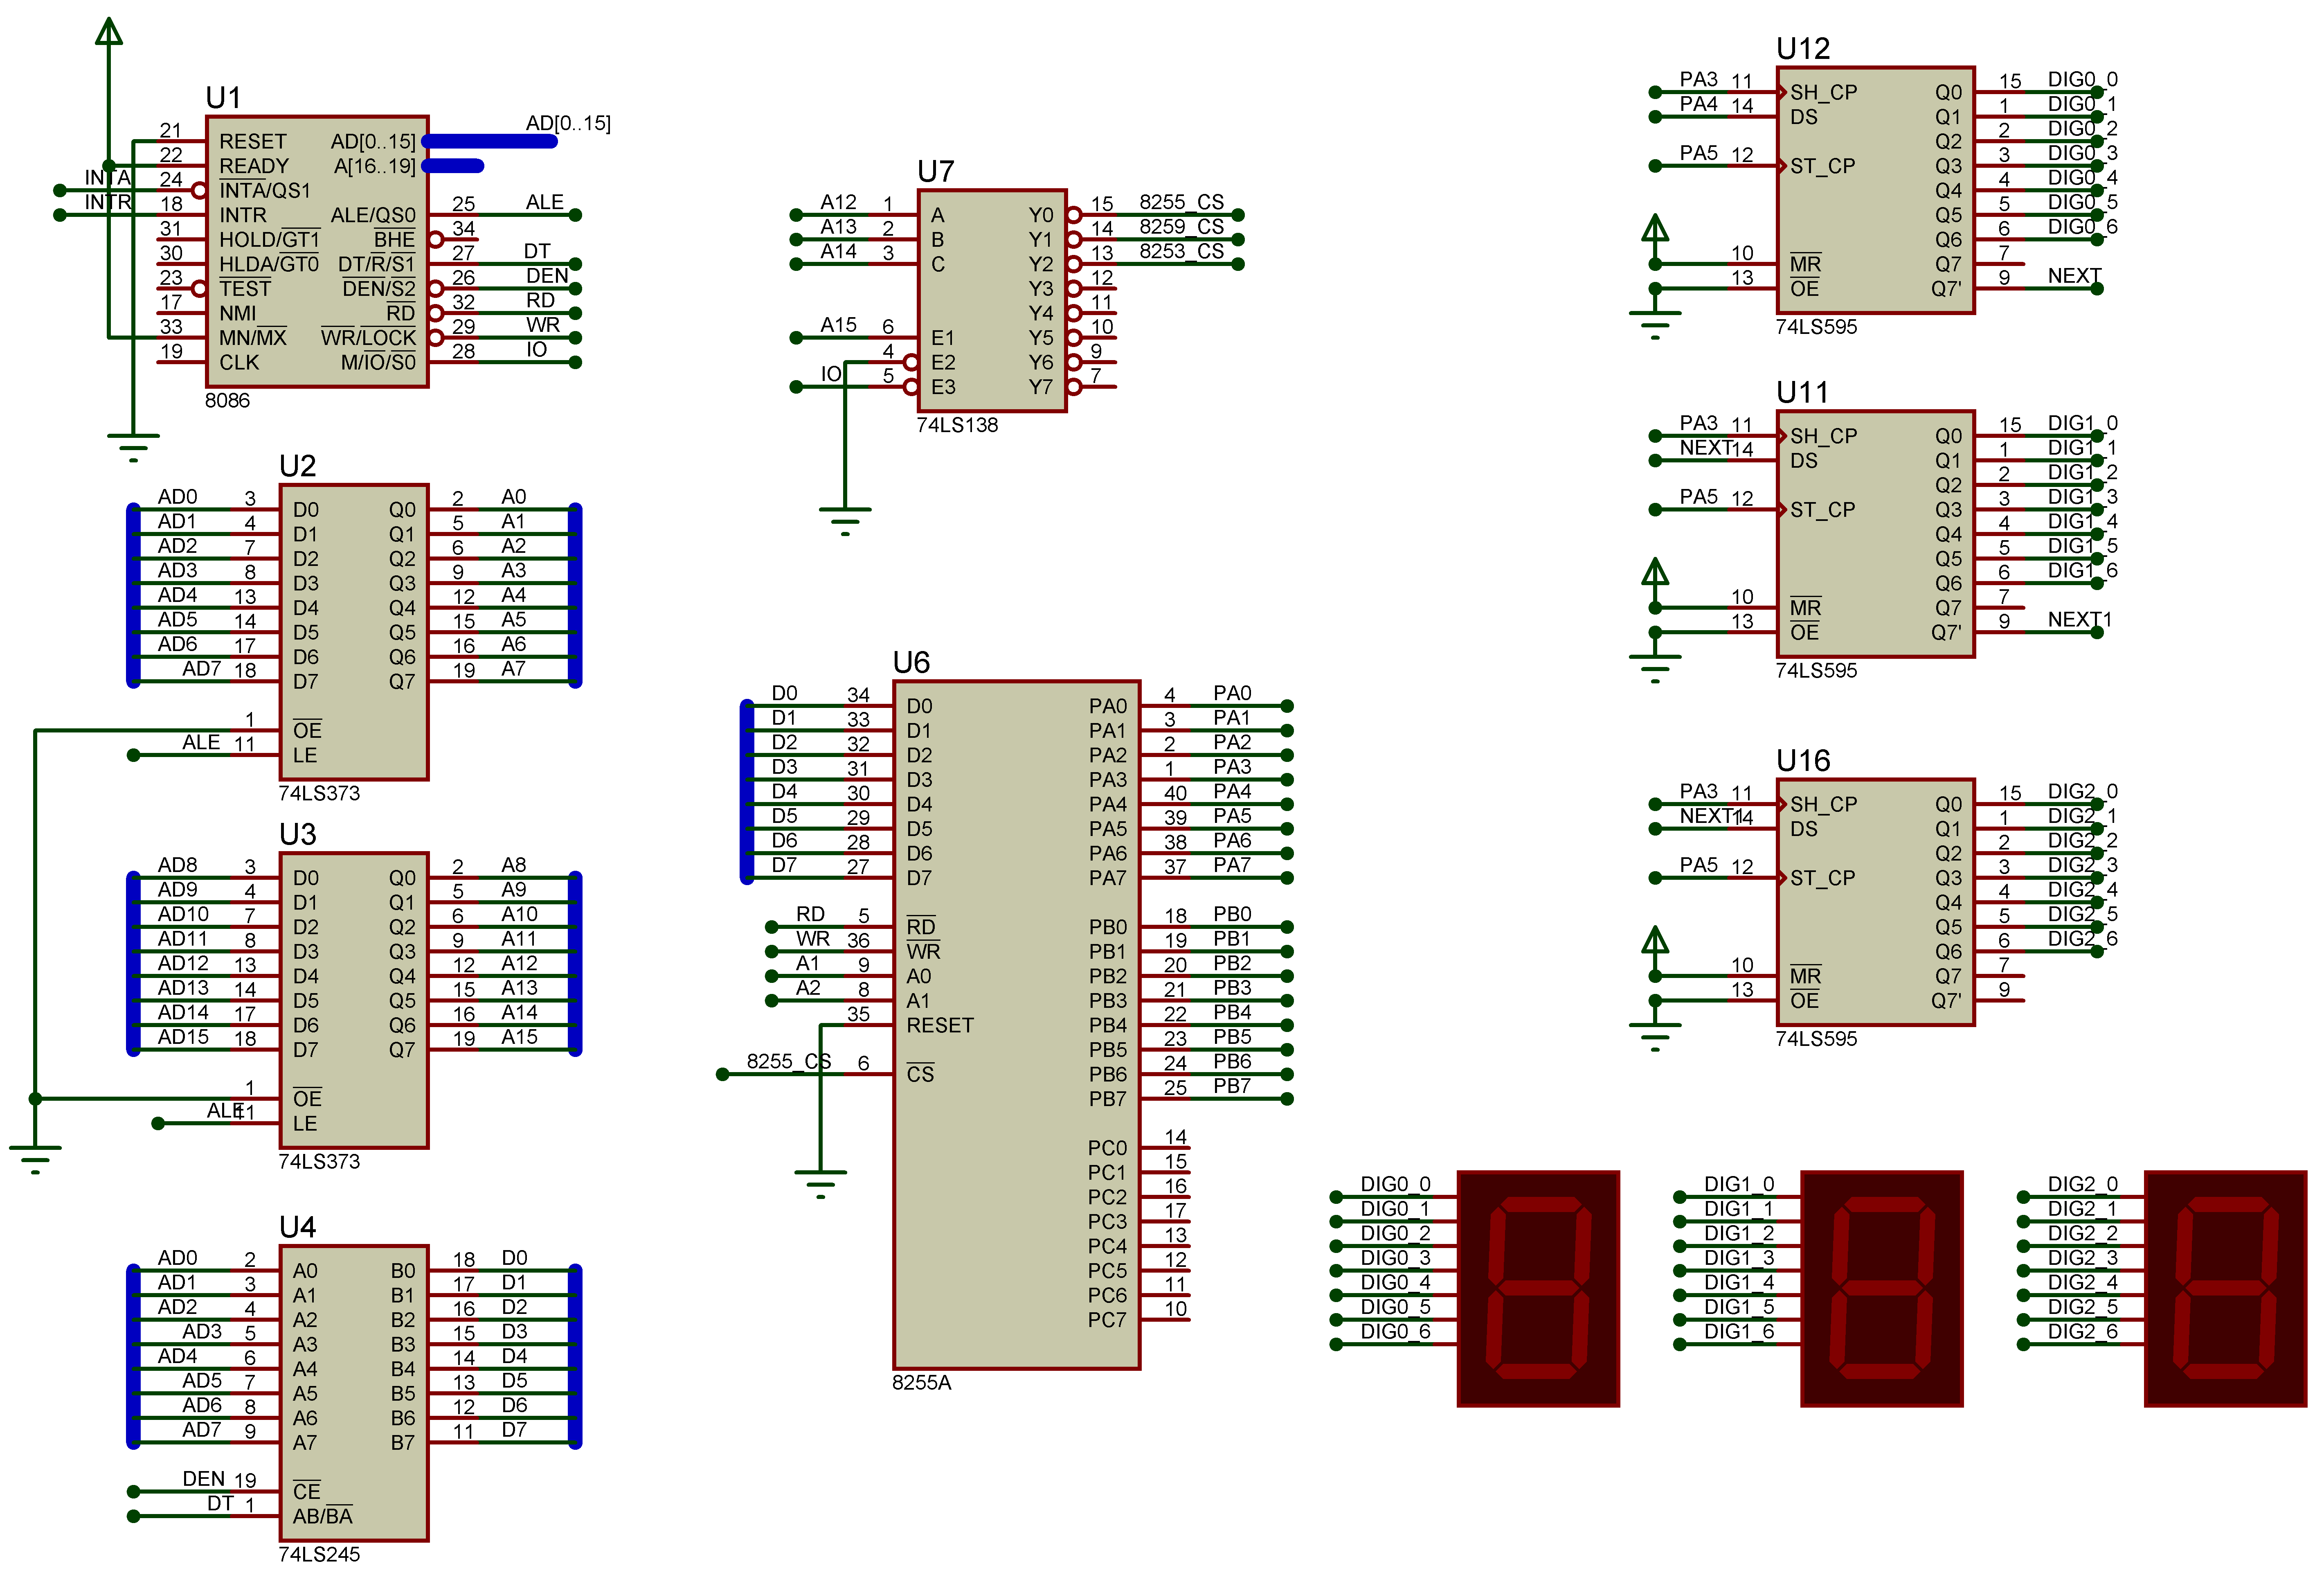
\includegraphics[width=0.5\textwidth]{../截图/数码管显示部分硬件设计}
				\caption{数码管显示部分原理图}
				\label{fig:数码管显示部分硬件设计}
			\end{figure}
			
			该部分，信号从8086输出后，经过8255的PA并行接口的引脚PA3、PA4、PA5三根信号线输出给74LS595，74LS595接收端从图\ref{fig:74LS595内部框图}中可以看出是一个8比特的移位寄存器，从$SER$引脚输入，至$Q7'$引脚输出，单独芯片完成8位数据收发
			
			仿真采用7位共阴极数码管，对于小数点$dp$位并没有固定要求，其七段码对应如表\ref{tab:共阴极数码管七段码}，本芯片与MAX7219共用8255芯片，因此地址保持不变，详见表\ref{tab:8255芯片的外设地址}所示。
			\begin{table}[h!]
				\centering
				\caption{共阴极数码管七段码}
				\begin{tabular}{c|c|c}
					数字 & 二进制七段码 & 采用值\\
					\hline\hline
					0   & 1111 110xB & 0FCH\\
					1   & 0110 000xB & 060H\\
					2   & 1101 101xB & 0DAH\\
					3   & 1111 001xB & 0F2H\\
					4   & 0110 011xB & 066H\\
					5   & 1011 011xB & 0B6H\\
					6   & 1011 111xB & 0BEH\\
					7   & 1110 000xB & 0E0H\\
					8   & 1111 111xB & 0FEH\\
					9   & 1111 011xB & 0F6H
				\end{tabular}
				\label{tab:共阴极数码管七段码}
			\end{table}
		\subsection{按键输入部分}	
			按键部分采用8255作为驱动，其原理图如图\ref{fig:按键输入部分硬件设计}所示。
			\begin{figure}[H]
				\centering
				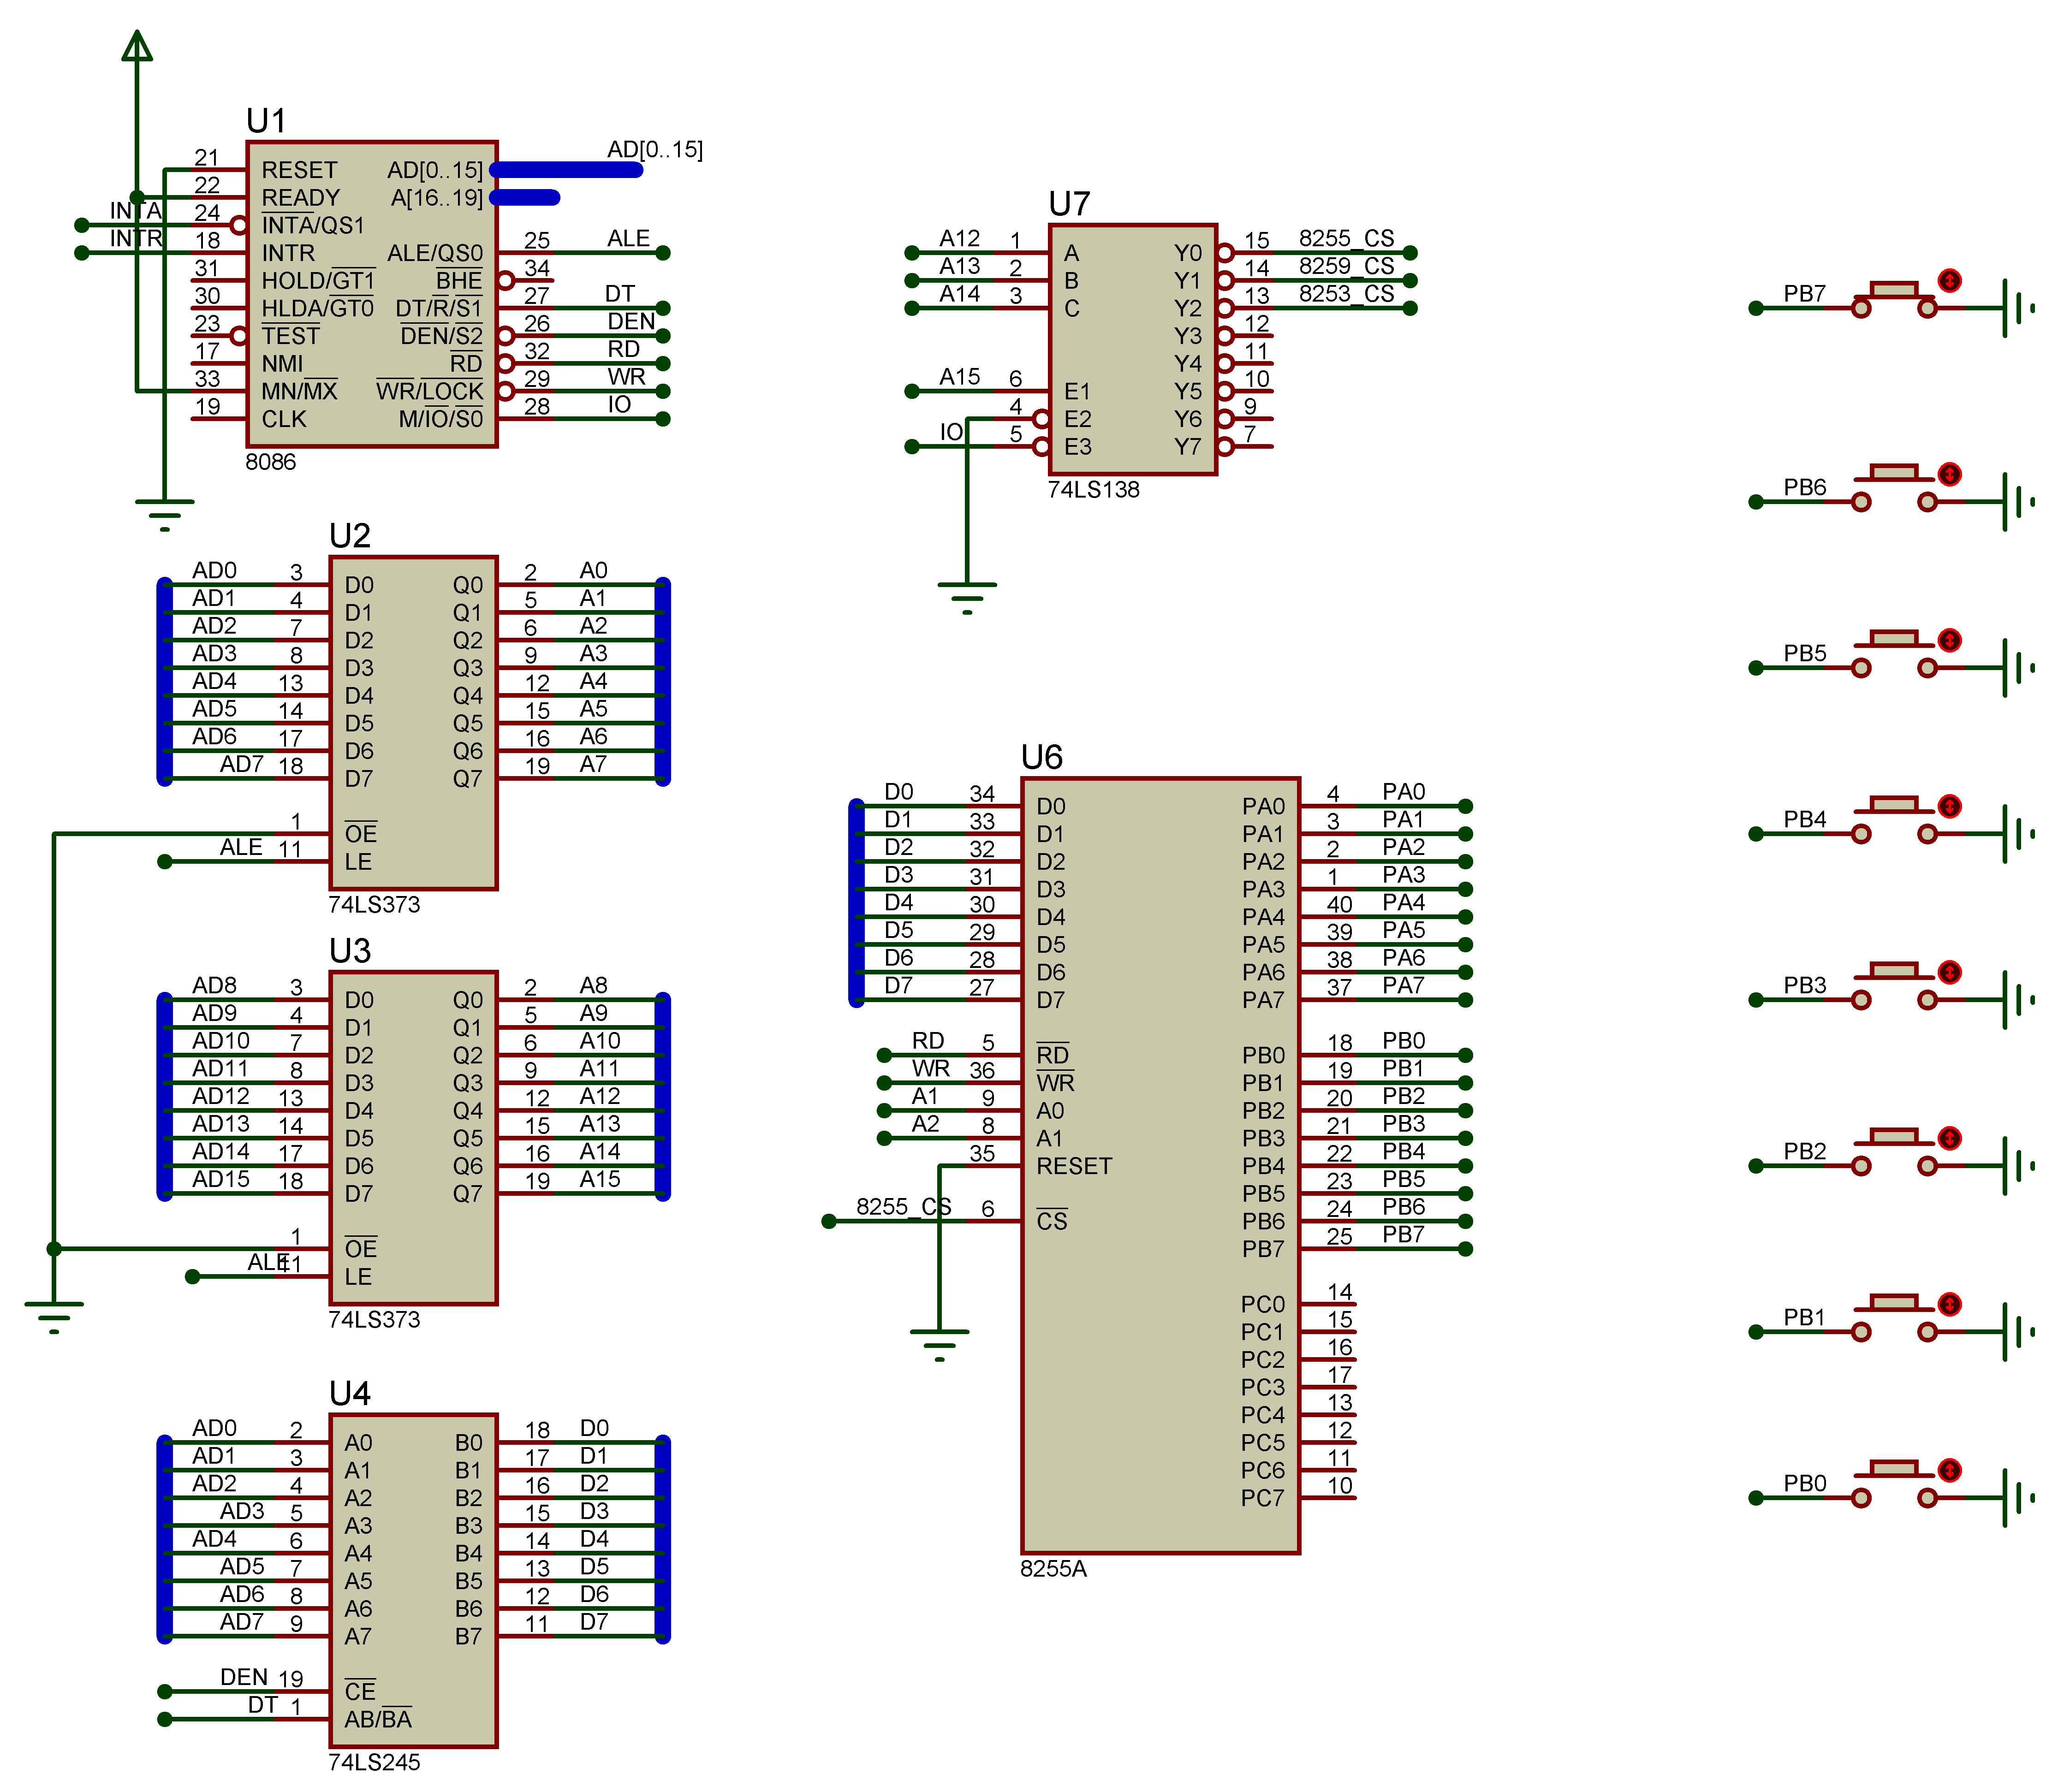
\includegraphics[width=0.5\textwidth]{../截图/按键输入部分硬件设计}
				\caption{按键输入部分原理图}
				\label{fig:按键输入部分硬件设计}
			\end{figure}
			
			该部分按键通过8255的PB口输入，由于仿真软件在8255的PB口中自带上拉电阻，因此只需要设计接地的按键便可完成设计。
			
			同时，按键部分与MAX7219共用8255芯片，因此地址保持不变，详见表\ref{tab:8255芯片的外设地址}所示。
	\newpage
	\section{软件设计}
		整体流程图如图\ref{fig:总体流程图}所示。
		\begin{figure}[H]
			\centering
			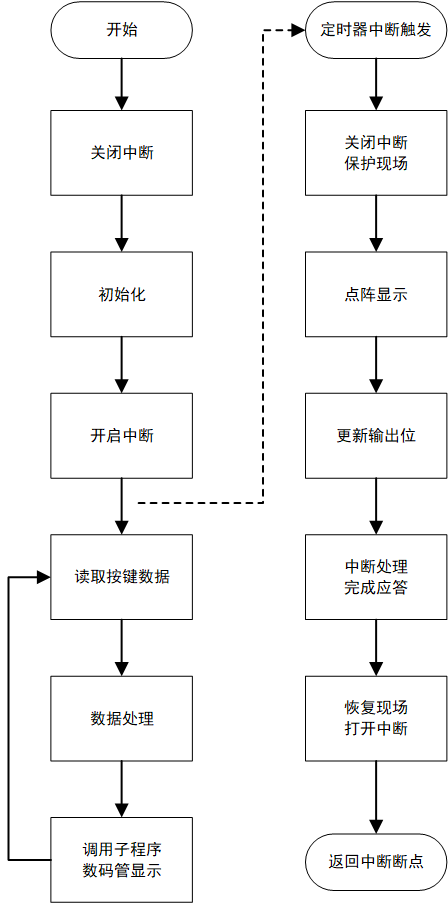
\includegraphics[width=0.5\textwidth]{../截图/总体流程图}
			\caption{总体流程图}
			\label{fig:总体流程图}
		\end{figure}
		整体流程大致可分为三个部分：
		\begin{compactenum}
			\item 各芯片初始化部分；
			\item 主循环部分；
			\item 定时器中断部分。
		\end{compactenum}
		首先，8086会屏蔽中断，执行各芯片初始化部分，初始化后打开中断，若中断触发，则执行定时器中断部分的点阵显示中文循环，否则执行主循环部分，读取按键后，将二进制译作十进制后再数码管中显示。
		
		如下，将对每个部分的设计一一作出详细介绍。
		\subsection{各芯片初始化部分}
			各芯片初试化部分需要对5块芯片以及中断向量表初始化，具体流程如下图\ref{fig:初始化流程图}所示。
			\begin{figure}[H]
				\centering
				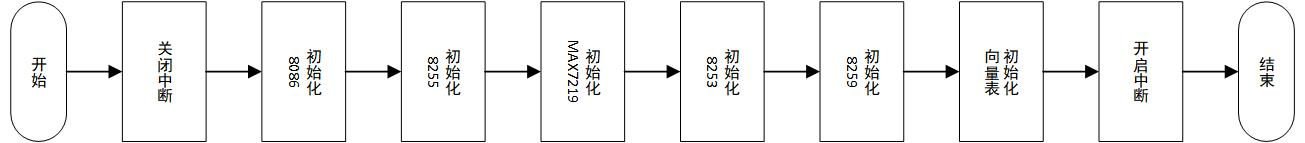
\includegraphics[width=0.95\textwidth]{../截图/初始化流程图}
				\caption{初始化流程图}
				\label{fig:初始化流程图}
			\end{figure}
			第一步关闭中断，指使用CLI指令屏蔽可屏蔽中断。
			
			第二步初始化8086，指为8086芯片的数据段寄存器（DS），堆栈段寄存器（SS）和附加段寄存器（ES）赋初值。
			
			第三步初始化8255，选择8255的控制字地址（可查表\ref{tab:8255芯片的外设地址}）:8006H，为该寄存器复制82H，表明A口工作模式0，输出；B口工作模式0，输入；C口均作为输出。
			
			第四步初始化MAX7219，调用MAX7219初始化子程序完成，该函数针对图\ref{fig:MAX7219寄存器地址图}中给出的地址为0xX9-0xXC，0xXF的寄存器分别赋值。由于四片串联，且为了保证四个点阵显示条件相同，因此直接连续四次写入相同的地址和数据后拉起寄存器输入信号引脚。方便初始化，也便于代码编写。具体寄存器作用在该芯片的数据芯片中已经给出，使用含义在附录中的代码后也以注释形式注明。
			
			第五步初始化8253，按照图\ref{fig:8253初始化编程顺序}中给出的初始化顺序，根据表\ref{tab:8253芯片的外设地址}中给出的外设地址，先向控制字地址A006H，先后申请打开计数器0和计数器1，随后向计数器0地址A000H和计数器1地址A002H写入对应分频系数。但此处需要说明的是，由于仿真软件Proteus的时间流速和客观时间的流速是不一致的，因此为了快速得到相关的实验现象需要将分频系数降低，也就是定时器中断时间简短。基于仿真环境的时间流速和芯片最高传输速率的考量，最终选择计数器0的计数值为6FH，计数器1的计数值为4FH。
			
			第六步初始化8259，按照图\ref{fig:8259A初始化编程顺序}中给出的初始化顺序和硬件图，判断出不必写入级联控制字ICW3，随后按照表\ref{tab:8259A芯片的外设地址}中给出的控制字地址，向初始化字ICW1中写入单片中断以及上升沿触发，中断向量码ICW2中写入中断向量码为60H-67H，跳过级联控制字ICW3后，向中断方式结束字ICW4中写入一般嵌套、非缓冲模式。由于八条中断线只使用一条，因此还需要提交操作命令字OCW1，频率高六位中断。
			
			第七步初始化中断向量表，首先建立中断服务函数INT0，随后根据向量表建立在段基地址为0H的规则，向附加段寄存器（ES）中赋值0H，以方便向量表的写入。根据第六步中中断向量码ICW2中所写起始地址60H，和硬件中中断信号连入IR0，计算得到对应中断服务函数的IP地址应当写入首地址为60H$\times$4H的字中，CS地址应当写入首地址为60H$\times$4+2H的字中。
			
			第八步打开中断，指使用STI指令开启可屏蔽中断。
			
			以上八个步骤完成了整体系统的初始化，接下来将在定时器中断信号中进行主函数的循环。
		\subsection{主循环部分}
			主循环部分功能主要是读取按键，将其对应2-10进制转换后输出至数码管即可。具体流程如下图\ref{fig:主循环流程图}所示。
			\begin{figure}[H]
				\centering
				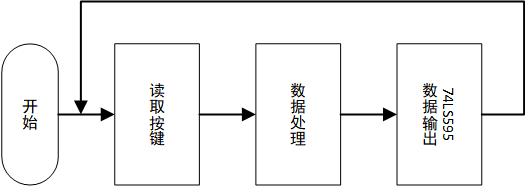
\includegraphics[width=0.50\textwidth]{../截图/主循环流程图}
				\caption{主循环流程图}
				\label{fig:主循环流程图}
			\end{figure}
			第一步，读取按键输入，该步只需要读取对应的PB口输入即可，PB寄存器地址已在表\ref{tab:8255芯片的外设地址}中给出。
			
			第二步，数据处理，由于采用的是上拉电阻的方案，因此得到的数据采用反逻辑编码，与人们所熟知的正逻辑相悖，因此需要使用NOT指令转换逻辑。
			
			第三步，调用DIGITAL$\_$OUTPUT子程序输出。该子程序将需要处理的数据按十进制分为个位、十位、百位。查表\ref{tab:共阴极数码管七段码}，得到对应七段码，按低位优先的顺序，逐个推入74LS595芯片中。
			
			完成以上三步后，进行无条件跳转，用以实现主函数的死循环。
		\subsection{定时器中断部分}
			定时器中断部分功能主要是控制点阵输出，并计算下一次中断点阵显示字的序号。具体流程如下图\ref{fig:定时器中断流程图}所示。
			\begin{figure}[H]
				\centering
				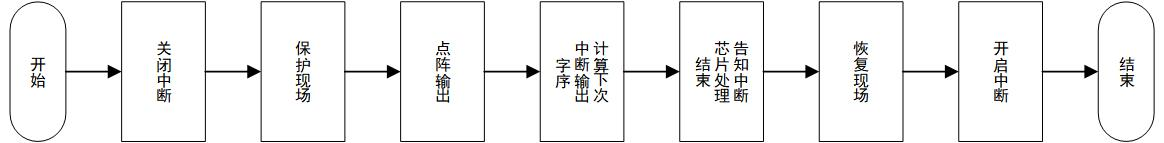
\includegraphics[width=0.50\textwidth]{../截图/定时器中断流程图}
				\caption{定时器中断流程图}
				\label{fig:定时器中断流程图}
			\end{figure}
			第一步，关闭中断，使用CLI指令屏蔽可屏蔽中断。
			
			第二步，保护现场，由于中断的指令将会充分使用四个数据寄存器，且中断时刻无法确定主函数正在执行哪条语句，因此，需要将四个数据寄存器的内容都分别推送入栈中，加以保护。
			
			第三步，点阵输出，首先需要从数据段中找出所要输出汉字的汉字码信息，并且由于数据量较大，因此应当选用基址变址相对寻址方式进行，但可惜本文由于时间关系并没有很好的做到这个方案，而是先将变址与相对地址相加，在和基址一并查表得出，实现了既定目标，但是代码较为杂乱。接着是点阵输出的主要方法是行选，因为loop指令是CX截止到0H时停止循环运行，因此，此处从高位行往低位行扫描是一个较为良好的方案。每次推送四个点阵的最低位数据随后拉起信号线。以此重复八次后，得到了一个完整字的全部输出，也就完成了点阵输出。
			
			第四步，计算下次中断输出，其本质是对计数器CHAR$\_$NUMBER进行加1操作，但是需要注意的是，需要对最后一位跳转到第一位这个边界条件进行一定的条件运算处理。本文给出直接与总字数作比的方案，随后考察CF标志位的方案。
			
			第五步，告知中断芯片处理结束，使得下次中断得以正常接收。本质是写中断结束操作命令字OCW2，向其写入中断结束指令。
			
			第六步，恢复现场，将保护现场中的内容取出，使得主函数的数据恢复。
			
			第七步，打开中断，使用STI指令开启可屏蔽中断。
			
			以上七步构成完整的定时器中断。
			
	\newpage
	\section{现象演示}
		\subsection{点阵现象}
			点阵由定时器中断控制，循环显示“检测二班游寅龙”七个字，如图\ref{fig:点阵显示}。
			\begin{figure}[h]
				\centering
				\begin{subfigure}{0.22\linewidth}
					\centering
					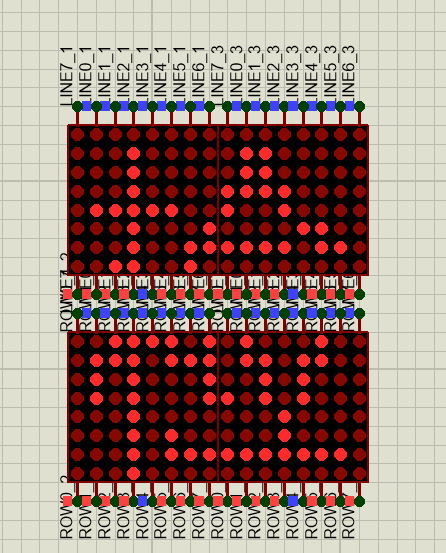
\includegraphics[width=0.9\linewidth]{../截图/检字}
					\caption{“检”字}
				\end{subfigure}
				\begin{subfigure}{0.22\linewidth}
					\centering
					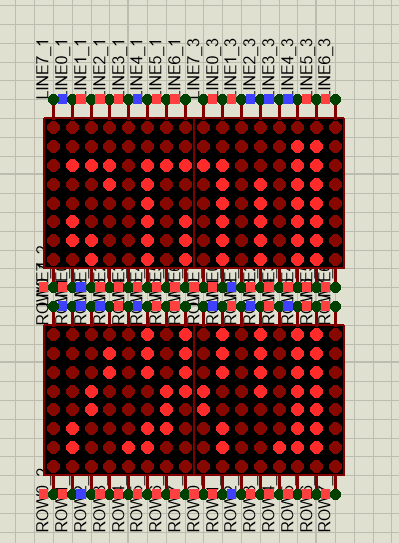
\includegraphics[width=0.9\linewidth]{../截图/测字}
					\caption{“测”字}
				\end{subfigure}
				\begin{subfigure}{0.22\linewidth}
					\centering
					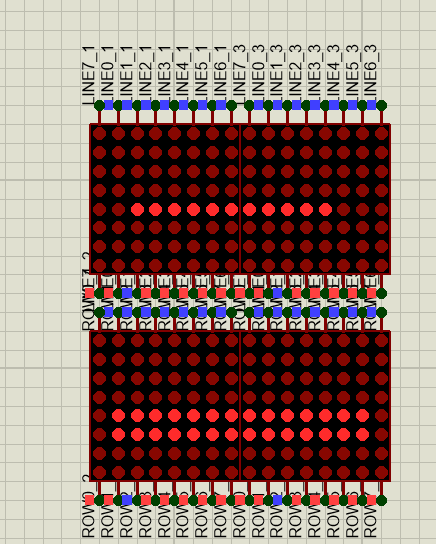
\includegraphics[width=0.9\linewidth]{../截图/二字}
					\caption{“二”字}
				\end{subfigure}
				\begin{subfigure}{0.22\linewidth}
					\centering
					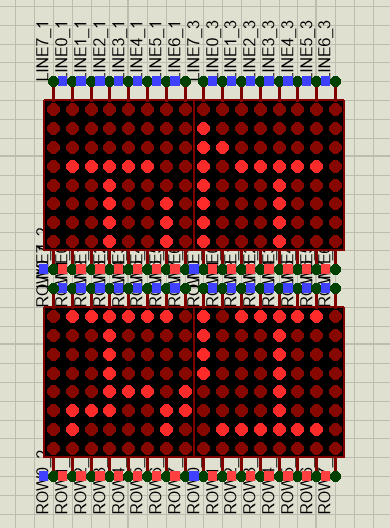
\includegraphics[width=0.9\linewidth]{../截图/班字}
					\caption{“班”字}
				\end{subfigure}
				\centering
				\begin{subfigure}{0.22\linewidth}
					\centering
					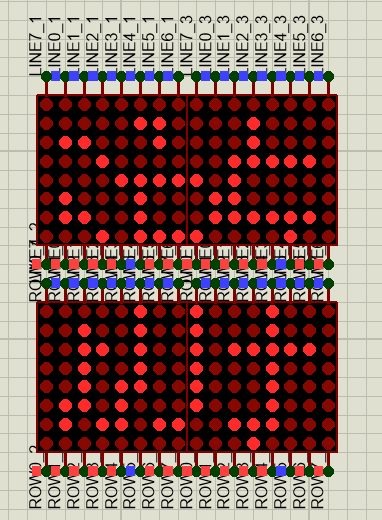
\includegraphics[width=0.9\linewidth]{../截图/游字}
					\caption{“游”字}
				\end{subfigure}
				\begin{subfigure}{0.25\linewidth}
					\centering
					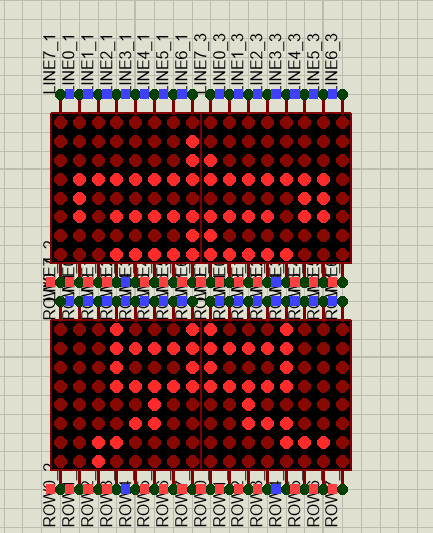
\includegraphics[width=0.9\linewidth]{../截图/寅字}
					\caption{“寅”字}
				\end{subfigure}
				\begin{subfigure}{0.25\linewidth}
					\centering
					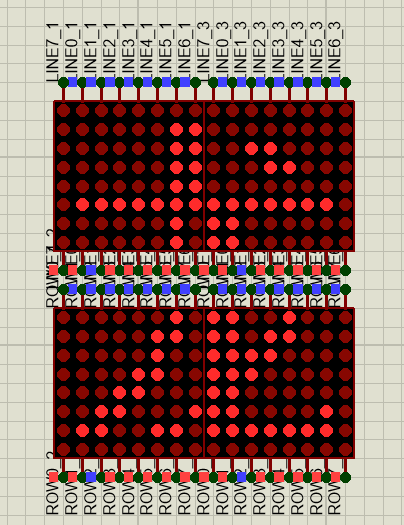
\includegraphics[width=0.9\linewidth]{../截图/龙字}
					\caption{“龙”字}
				\end{subfigure}
				
				\caption{点阵七位汉字显示}
				\label{fig:点阵显示}
			\end{figure}
			
			此现象证明定时器中断部分代码正确，同时也说明了代码为本人所著。
		\subsection{数码管现象}
			数码管数字为按键的二进制转换，按人们习惯，按键按下记为1，按键断开记为0。以下试举两例，如图\ref{fig:数码管显示}。
			\begin{figure}[h]
				\centering
				\begin{subfigure}{0.45\linewidth}
					\centering
					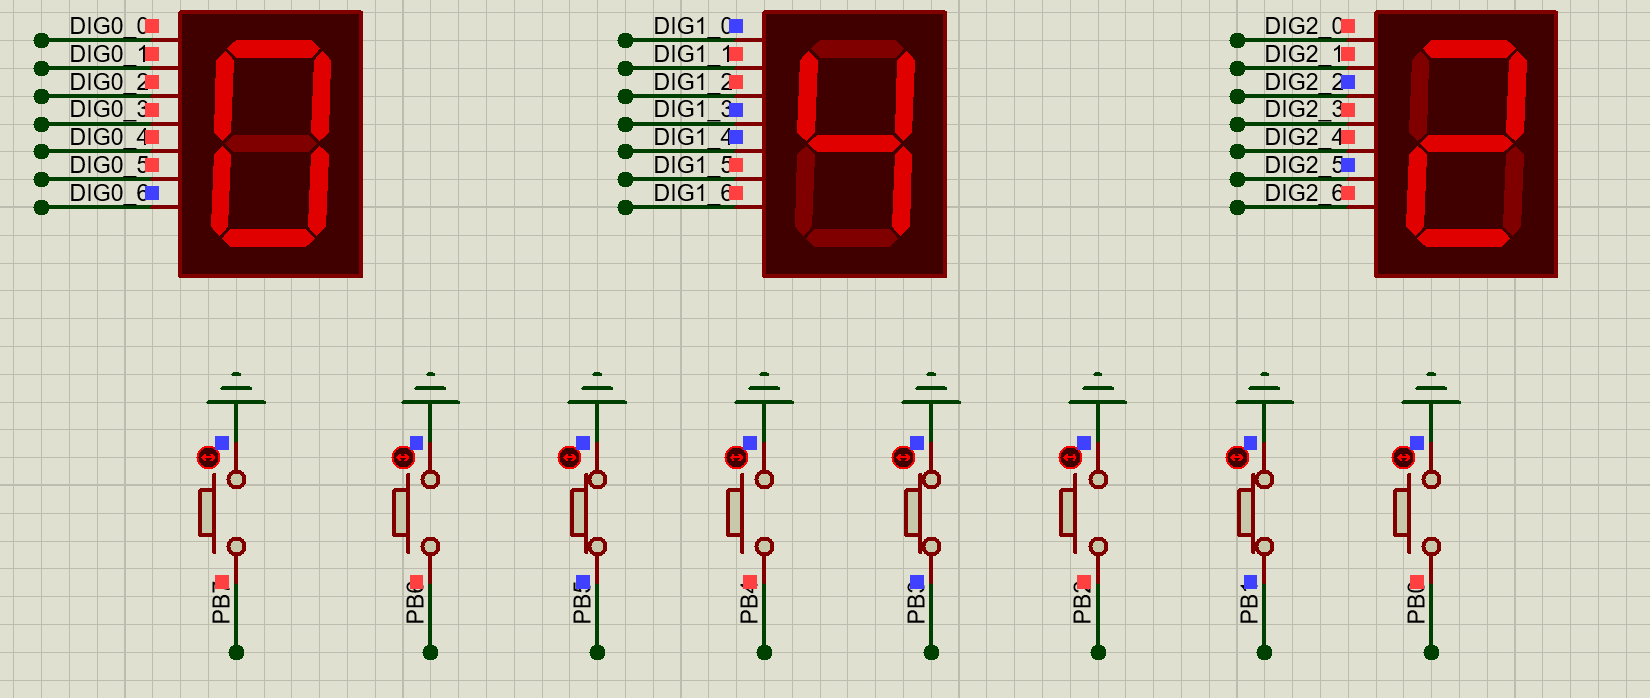
\includegraphics[width=0.9\linewidth]{../截图/数码管1}
					\caption{数码管示例1}
				\end{subfigure}
				\begin{subfigure}{0.45\linewidth}
					\centering
					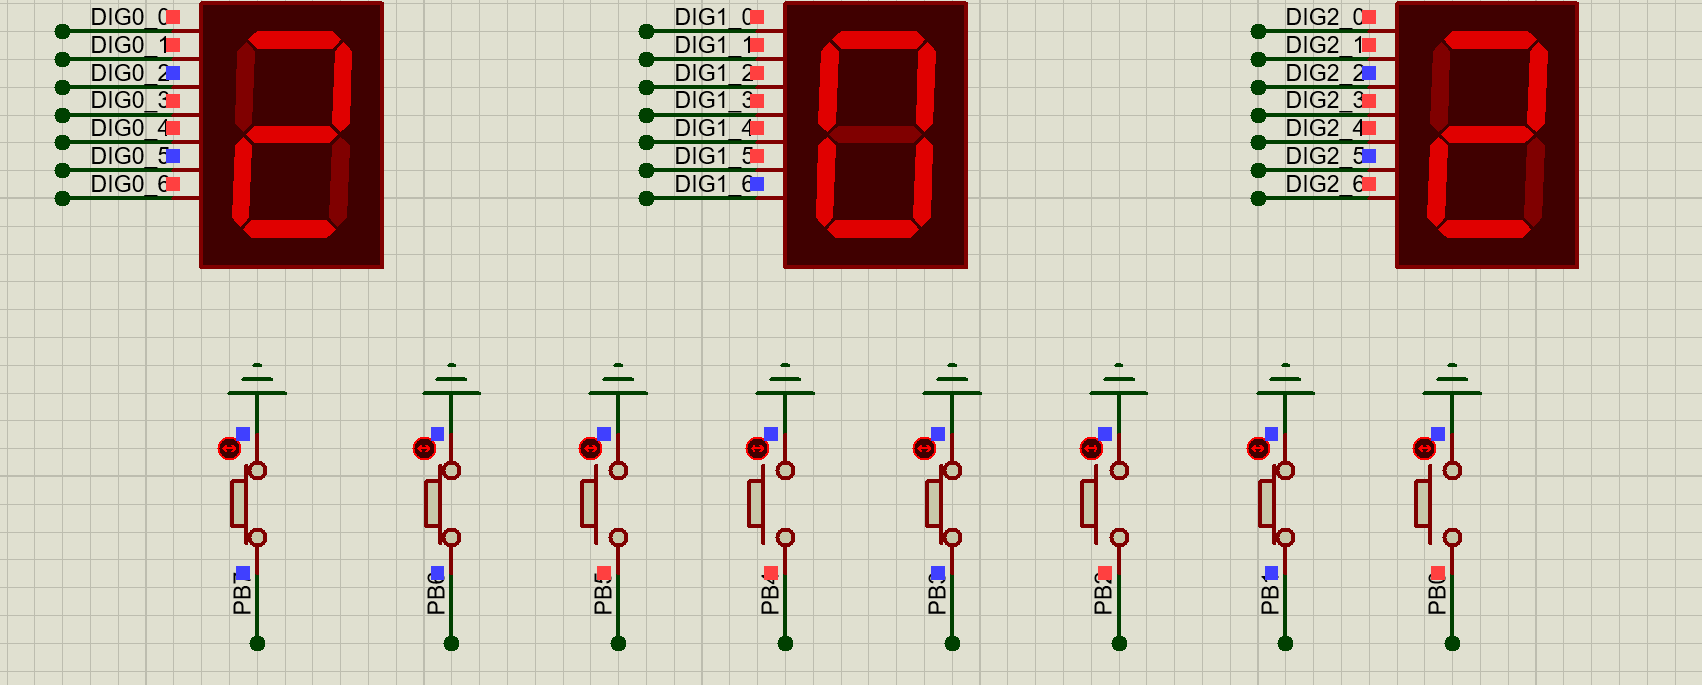
\includegraphics[width=0.9\linewidth]{../截图/数码管2}
					\caption{数码管示例2}
				\end{subfigure}
				\caption{数码管译码举例示范}
				\label{fig:数码管显示}
			\end{figure}
			
			对比按键所示二进制和数码管显示十进制，两者表达同一数字，证明主函数部分代码正确。
	\newpage
	\section{总结}
		自从我深入探索微机原理的世界，我对计算机科学的理解达到了一个新的高度。这不仅仅是一门学科的学习，更是一次自我挑战和成长的旅程。
		
		随着课程的深入，我逐渐感受到了计算机科学的魅力。从最初的CPU、内存、I/O设备等基础概念，到后来的指令系统、存储系统、输入输出系统等复杂知识，每一步的学习都让我对计算机有了更深刻的认识。
		
		在学习CPU的内部结构和工作流程时，我被其设计的精妙所震撼。它像一个高效的工厂，通过执行各种指令来完成复杂的计算任务。这让我深刻体会到，计算机科学不仅仅是理论的学习，更是对实际应用的深入理解和探索。
		
		在编写汇编程序的过程中，我亲身体验了从高级语言到机器语言的转换过程。这一过程让我对计算机程序的工作原理有了更直观的认识。同时，我也意识到编程不仅仅是一种技能，更是一种思维方式的训练。它要求我们具备严密的逻辑思维和解决问题的能力。
		
		在本次的大作业中，我也亲手结合硬件和软件，搭建了8086处理系统，虽然因为时间的原因，这个系统不管是从硬件角度还是软件都有很多的提升改进之处，但是这次大作业让我深刻对微机的工作方式有了理解，对于芯片之间的连接控制有了更系统的了解，也扩展了我的眼界。
		
		总的来说，微机原理的学习让我对计算机科学有了更深入的理解。我不仅掌握了相关的知识和技能，还培养了严密的逻辑思维和解决问题的能力。我相信，在未来的学习和工作中，我将继续深入探索微机原理的奥秘，为计算机科学的发展贡献自己的力量。同时，我也希望能够将这些知识应用到实际中，为社会的发展做出自己的贡献。
			
    \newpage
	\bibliography{IEEEabrv,bib/tex}
	\newpage
	
	\zihao{-3}\bfseries\centering{附 \space 录（程序清单）}
	\mdseries
\begin{lstlisting}[language={[x86masm]Assembler}]
DATASE SEGMENT
	C8253CTRL  EQU 0A006H
	C8253A	   EQU 0A000H
	C8253B	   EQU 0A002H
	C8253C	   EQU 0A004H		;8253地址
	
	C8255CTRL  EQU 08006H
	C8255A	   EQU 08000H
	C8255B	   EQU 08002H
	C8255C	   EQU 08004H		;8255地址
	
	C8259ICW1  EQU 09000H
	C8259ICW2  EQU 09002H
	C8259ICW3  EQU 09002H
	C8259ICW4  EQU 09002H		;8259A初始化命令字地址
	
	C8259OCW1  EQU 09002H
	C8259OCW2  EQU 09000H
	C8259OCW3  EQU 09000H		;8259A操作命令字地址
	
	
	MAX7219_ADDR  DB 00H		;待访问的MAX7219寄存器地址（MAX7219_WRITE_DATA调用）
	MAX7219_DATA  DB 00H		;待访问的MAX7219寄存器数据（MAX7219_WRITE_DATA调用）
	MAX7219_DIN_H	   EQU 02H	;CS=0 DIN=1 CLK=0  (INC DIN_H能使得时钟线拉高)
	MAX7219_DIN_L	   EQU 00H	;CS=0 DIN=0 CLK=0  (INC DIN_L能使得时钟线拉高)
	MAX7219_CS_H 	   EQU 04H	;CS=1
	
	LS595_OUTPUT DB 00H		;待74LS595输出的数据（DIGITAL_OUTPUT调用）
	LS595_DAT_H EQU 14H		;RCK=0 DAT=1 SCK=0 (ADD DAT,08H能使得时钟线拉高)
	LS595_DAT_L EQU 04H		;RCK=0 DAT=0 SCK=0 (ADD DAT,08H能使得时钟线拉高)
	LS595_RCK_H EQU 24H		;RCK=1
	LS595_RCK_L EQU 04H		;RCK=0
	
	CHAR_NUMBER DB 00H		;指示点阵下一个显示的字（INT0调用）
	
	DIGITAL_NUM 	;共阴极数码管字库,每个字节代表一个阿拉伯数字
	DB 0FCH,060H,0DAH,0F2H,66H,0B6H,0BEH,0E0H,0FEH,0F6H;
	
	NAME_CHAR	;点阵字库,每两行代表一个字, "检测二班游寅龙"	
	DB 000H,010H,010H,010H,07CH,011H,013H,032H,03DH,077H,051H,051H,010H,014H,017H,010H;
	DB 000H,060H,060H,0F0H,090H,00CH,0F6H,000H,044H,06CH,028H,0A8H,010H,010H,0FEH,000H;
	DB 000H,000H,077H,014H,004H,045H,065H,025H,005H,015H,015H,023H,022H,046H,04CH,000H;
	DB 000H,006H,0C6H,056H,056H,056H,056H,056H,056H,056H,056H,096H,086H,046H,04EH,000H;
	DB 000H,000H,000H,000H,03FH,000H,000H,000H,000H,000H,000H,000H,07FH,07FH,000H,000H;
	DB 000H,000H,000H,000H,0F8H,000H,000H,000H,000H,000H,000H,000H,0FEH,0FEH,000H,000H;
	DB 000H,000H,000H,07CH,010H,012H,012H,012H,07EH,010H,010H,010H,01DH,073H,042H,000H;
	DB 000H,080H,0C0H,0BEH,088H,088H,088H,088H,0BEH,088H,088H,088H,008H,008H,07EH,000H;
	DB 000H,006H,062H,010H,00FH,044H,064H,017H,004H,024H,034H,024H,02CH,068H,05BH,000H;
	DB 000H,010H,010H,03EH,0A0H,060H,07EH,084H,088H,088H,0BEH,088H,088H,088H,038H,010H;
	DB 000H,001H,001H,07FH,040H,05FH,001H,01FH,011H,01FH,011H,01FH,004H,00CH,030H,020H;
	DB 000H,000H,080H,0FEH,006H,0F6H,080H,0F8H,088H,0F8H,088H,0F8H,020H,038H,00EH,000H;
	DB 000H,003H,003H,003H,003H,07FH,002H,002H,002H,006H,004H,00CH,018H,031H,066H,000H;
	DB 000H,000H,030H,018H,000H,0FEH,0C0H,0C0H,0C8H,0D8H,0F0H,0E0H,0C0H,0C2H,0FEH,000H;
DATASE ENDS

STACKSE SEGMENT STACK
	DW 256H DUP(?)
STACKSE ENDS

EXTRASE	SEGMENT
	DW 256H DUP(?)
EXTRASE	ENDS

CODESE  SEGMENT PUBLIC 'CODE'
;;;;;;;;主函数;;;;;;;;
	MAIN	PROC
		ASSUME CS:CODESE, DS:DATASE, SS:STACKSE, ES:EXTRASE
	START:
		CLI			;关闭中断
		
		MOV AX, DATASE
		MOV DS, AX
		MOV AX, STACKSE
		MOV SS, AX
		MOV AX, EXTRASE
		MOV ES, AX		;段寄存器赋值
		
		MOV DX, C8255CTRL
		MOV AL, 10000010B
		OUT DX, AL		;8255初始化——A口输出，B口输入
		
		CALL MAX7219_INIT	;调用子程序初始化MAX7219
		
		MOV DX, C8253CTRL
		MOV AL, 00010110B
		OUT DX, AL		;8253初始化——打开计数器0
		
		MOV DX, C8253CTRL
		MOV AL, 01010110B
		OUT DX, AL		;8253初始化——打开计数器1
		
		MOV DX, C8253A 
		MOV AL, 006FH
		OUT DX, AL		;8253初始化——计数器0计数6FH
		
		MOV DX, C8253B
		MOV AL, 04FH
		OUT DX, AL		;8253初始化——计数器0计数4FH
		
		MOV DX, C8259ICW1
		MOV AL, 00010011B
		OUT DX, AL		;8259A初始化——设置为单片上升沿触发
		
		MOV DX, C8259ICW2
		MOV AL, 060H
		OUT DX, AL		;8259A初始化——设置IR0-IR7对应中断向量60H-67H
		
		MOV DX, C8259ICW4
		MOV AL, 00000001B
		OUT DX, AL		;8259A初始化——设置为一般嵌套、非缓冲
		
		MOV DX, C8259OCW1
		MOV AL, 11111100B
		OUT DX, AL		;8259A初始化——屏蔽高六位中断，只保留IR0、IR1
		
		MOV AX, 00H
		MOV ES, AX		;定义中断向量表——附加段段基地址指向向量表段基地址
		
		MOV BX, 60H*4
		MOV AX, OFFSET INT0
		MOV ES:[BX], AX		;定义中断向量表——写入中断服务函数的偏移地址
	
		MOV AX, CS
		MOV ES:[BX+2], AX	;定义中断向量表——写入中断服务函数的段基地址
		
		STI			;开启中断
		
	LOOP_C:
		MOV DX,C8255B
		IN  AL,DX		;读取按键数据
		
		NOT AL			;由于按键采用反逻辑，因此需要改为正逻辑
		
		MOV LS595_OUTPUT,AL
		CALL DIGITAL_OUTPUT	;将二进制交予数码管处理函数处理
		
		JMP LOOP_C		;跳回主函数形成死循环，防止停机
		
		RET			;实际运行不到，为了防止编译器给予警告
	MAIN ENDP
	
;;;;;;;;MAX7219初始化函数;;;;;;;;
	MAX7219_INIT PROC
		MOV MAX7219_ADDR, 09H
		MOV MAX7219_DATA, 00H	;译码方式设为不译码，地址0xX9，数值0x00
		CALL MAX7219_WRITE_DATA
		CALL MAX7219_WRITE_DATA
		CALL MAX7219_WRITE_DATA
		CALL MAX7219_WRITE_DATA	;四片芯片都是该译码方式
		MOV DX,C8255A
		MOV AL,MAX7219_CS_H
		OUT DX,AL		;传送结束，拉起片选信号
		
		MOV MAX7219_ADDR, 0AH	;亮度为7/32，地址0xXA，数值0xX3
		MOV MAX7219_DATA, 03H
		CALL MAX7219_WRITE_DATA
		CALL MAX7219_WRITE_DATA
		CALL MAX7219_WRITE_DATA
		CALL MAX7219_WRITE_DATA	;四片芯片都是该亮度
		MOV DX,C8255A
		MOV AL,MAX7219_CS_H
		OUT DX,AL		;传送结束，拉起片选信号
		
		MOV MAX7219_ADDR, 0BH
		MOV MAX7219_DATA, 07H	;扫描界限为8行，地址0xXB，数值0xX7
		CALL MAX7219_WRITE_DATA
		CALL MAX7219_WRITE_DATA
		CALL MAX7219_WRITE_DATA
		CALL MAX7219_WRITE_DATA	;四片芯片都是该扫描界限
		MOV DX,C8255A
		MOV AL,MAX7219_CS_H
		OUT DX,AL		;传送结束，拉起片选信号
		
		MOV MAX7219_ADDR, 0CH
		MOV MAX7219_DATA, 01H	;关断寄存器为普通模式，地址0xXC，数值0xX1
		CALL MAX7219_WRITE_DATA
		CALL MAX7219_WRITE_DATA
		CALL MAX7219_WRITE_DATA
		CALL MAX7219_WRITE_DATA	;四片芯片都是该普通模式
		MOV DX,C8255A
		MOV AL,MAX7219_CS_H
		OUT DX,AL		;传送结束，拉起片选信号
		
		MOV MAX7219_ADDR, 0FH
		MOV MAX7219_DATA, 00H	;显示器寄存器测试模式为关闭，地址0xXF，数值0xX0
		CALL MAX7219_WRITE_DATA
		CALL MAX7219_WRITE_DATA
		CALL MAX7219_WRITE_DATA
		CALL MAX7219_WRITE_DATA	;四片芯片都是该关闭模式
		MOV DX,C8255A
		MOV AL,MAX7219_CS_H
		OUT DX,AL		;传送结束，拉起片选信号
		
		RET			;返回原函数
	MAX7219_INIT ENDP
;;;;;;;;MAX7219单片数据写入;;;;;;;;
	MAX7219_WRITE_DATA PROC
		PUSH AX
		PUSH BX
		PUSH CX
		PUSH DX		;保护现场
		
		MOV DX,C8255A	;设置输出端口为8255的A口（DX以下不再变动）
		
		;按照芯片输出时序，先传送地址。
		MOV BL, MAX7219_ADDR	;传送地址入BX寄存器
		MOV CL, 08H		;计数器置为8（一个字节八位）
	ADDR_LOOP:
		TEST BL, 80H  		;将BL与80H求与，测试BL最高位是否是1
		JNZ ADDR_EQU_1		;跳转到传送低电平方案
		MOV AL, MAX7219_DIN_L
		JMP ADDR_EQU_0		;跳出分支结构
	ADDR_EQU_1:
		MOV AL, MAX7219_DIN_H
	ADDR_EQU_0:
		OUT DX, AL	;输出数据（此时时钟线为低）
		INC AL
		OUT DX, AL	;拉高时钟线并输出
		SHL BX, 01H	;左移，准备输出下一位
		LOOP ADDR_LOOP	;循环8次（每次传送一位）
		
		;按照芯片输出时序，再传送数据。
		MOV BL, MAX7219_DATA	;传送数据入BX寄存器
		MOV CL, 08H		;计数器置为8（一个字节八位）
	DATA_LOOP:
		TEST BL, 80H  		;将BL与80H求与，测试BL最高位是否是1
		JNZ DATA_EQU_1		;跳转到传送低电平方案
		MOV AL, MAX7219_DIN_L
		JMP DATA_EQU_0		;跳出分支结构
	DATA_EQU_1:
		MOV AL, MAX7219_DIN_H
	DATA_EQU_0:
		OUT DX, AL	;输出数据（此时时钟线为低）
		INC AL
		OUT DX, AL	;拉高时钟线并输出
		SHL BX, 01H	;左移，准备输出下一位
		LOOP DATA_LOOP	;循环8次（每次传送一位）
		
		POP DX
		POP CX
		POP BX
		POP AX		;恢复现场
		RET		;返回原函数
	MAX7219_WRITE_DATA ENDP
;;;;;;;;74LS595输出三位数;;;;;;;;
	DIGITAL_OUTPUT PROC FAR
		PUSH AX
		PUSH BX
		PUSH CX
		PUSH DX		;保护现场
		
		MOV DX, C8255A	;设置输出端口为8255的A口（DX以下不再变动）
		
		;先输出个位
		MOV AX, 00H		;将AH置0
		MOV AL, LS595_OUTPUT	;取出需要输出的三位数
		MOV BX, 10D
		DIV BL			;除以10（余数在AH，商在AL）
		PUSH  AX		;入栈（保留商，也就是十位和百位）
		MOV CL, 8H
		ROR AX, CL		;将余数（个位）移动至AL
		MOV BX, OFFSET DIGITAL_NUM	;取出数码管字库的数组首地址
		XLAT 			;查表（BX表示表格首地址，AL表示表内位移量）
		MOV BL, AL ;将数据放入BX寄存器（OUT指令只允许输出AX，判断需在BX中进行）
	OUPUT1_LOOP:
		TEST BL, 01H  		;将BL与80H求与，测试BL最高位是否是1
		JNZ OUPUT1_EQU_1	;跳转到传送高电平方案
		MOV AL, LS595_DAT_L
		JMP OUPUT1_EQU_0	;跳出分支结构
	OUPUT1_EQU_1:
		MOV AL, LS595_DAT_H
	OUPUT1_EQU_0:
		OUT DX, AL		;输出数据（此时时钟线为低）
		ADD AL, 08H		;拉高时钟线并输出
		OUT DX, AL 
		SHR BX, 01H		;右移，准备输出下一位
		LOOP OUPUT1_LOOP	;循环8次（每次传送一位）
		
		;随后输出十位
		POP AX			;取出上次除以10后的商和余数
		AND AX,00FFH		;清空AH（清空余数，只保留十位和百位的商）
		MOV BX, 10D
		DIV BL			;除以10（余数在AH，商在AL）
		PUSH  AX		;入栈（保留商，也就是百位）
		MOV CL, 8H
		ROR AX, CL		;将余数（十位）移动至AL
		MOV BX, OFFSET DIGITAL_NUM	;取出数码管字库的数组首地址
		XLAT 			;查表（BX表示表格首地址，AL表示表内位移量）
		MOV BL, AL ;将数据放入BX寄存器（OUT指令只允许输出AX，判断需在BX中进行）
	OUPUT2_LOOP:
		TEST BL, 01H  		;将BL与80H求与，测试BL最高位是否是1
		JNZ OUPUT2_EQU_1	;跳转到传送高电平方案
		MOV AL, LS595_DAT_L
		JMP OUPUT2_EQU_0	;跳出分支结构
	OUPUT2_EQU_1:
		MOV AL, LS595_DAT_H
	OUPUT2_EQU_0:
		OUT DX, AL		;输出数据（此时时钟线为低）
		ADD AL, 08H		;拉高时钟线并输出
		OUT DX, AL 
		SHR BX, 01H		;右移，准备输出下一位
		LOOP OUPUT2_LOOP	;循环8次（每次传送一位）
		
		;最后输出百位
		POP AX			;取出上次除以10后的商和余数
		MOV BX, OFFSET DIGITAL_NUM	;取出数码管字库的数组首地址
		XLAT 			;查表（BX表示表格首地址，AL表示表内位移量）
		MOV BL, AL ;将数据放入BX寄存器（OUT指令只允许输出AX，判断需在BX中进行）
		MOV CL, 8H		;计数器置为8（一个字节八位）
	OUPUT3_LOOP:
		TEST BL, 01H  		;将BL与80H求与，测试BL最高位是否是1
		JNZ OUPUT3_EQU_1	;跳转到传送高电平方案
		MOV AL, LS595_DAT_L
		JMP OUPUT3_EQU_0	;跳出分支结构
	OUPUT3_EQU_1:
		MOV AL, LS595_DAT_H
	OUPUT3_EQU_0:
		OUT DX, AL		;输出数据（此时时钟线为低）
		ADD AL, 08H		;拉高时钟线并输出
		OUT DX, AL 
		SHR BX, 01H		;右移，准备输出下一位
		LOOP OUPUT3_LOOP	;循环8次（每次传送一位）
		
		MOV AL, LS595_RCK_H
		OUT DX, AL  ;拉高存储时钟线，从移位寄存器转存带存储寄存器（相当于显示输出）
		
		MOV AL, LS595_RCK_L
		OUT DX, AL	;拉低存储时钟线，方便下一次输入数据
		
		POP DX
		POP CX
		POP BX
		POP AX		;恢复现场
		
		RET		;返回原函数
	DIGITAL_OUTPUT ENDP

;;;;;;;;定时器中断服务函数;;;;;;;;
	INT0 PROC 
		CLI		;关闭中断
		
		PUSH AX
		PUSH BX
		PUSH CX
		PUSH DX		;保护现场
		
		MOV AL,CHAR_NUMBER		;取出需要输出的汉字位
		MOV BL,32D
		MUL BL		;乘以32（一个汉字占32字节）
		MOV BX,OFFSET NAME_CHAR
		ADD BX,AX	;将点阵字库数组的地址加上汉字偏移
				;得到对应汉字存储数组的首地址（相当于基址变址相对寻址）
		
		MOV CX,08H		;计数器置为8（每个点阵八行）
	NEXT_CHAR:
		MOV MAX7219_ADDR, CL	;给与芯片寄存器地址
		
		MOV AL,CL
		ADD AL,23D		;推定第四个点阵需要显示的行值
		PUSH AX			;保存AL（方便其他点阵的推定）
		XLAT			;查表，获取第四个点阵需要输出的值
		MOV MAX7219_DATA, AL	
		CALL MAX7219_WRITE_DATA	;将输出值交由函数负责输出
		
		POP AX
		SUB AL,8H		;推定第三个点阵需要显示的行值
		PUSH AX			;保存AL（方便其他点阵的推定）
		XLAT			;查表，获取第三个点阵需要输出的值
		MOV MAX7219_DATA, AL
		CALL MAX7219_WRITE_DATA	;将输出值交由函数负责输出
		
		POP AX
		SUB AL,8H		;推定第二个点阵需要显示的行值
		PUSH AX			;保存AL（方便其他点阵的推定）
		XLAT			;查表，获取第二个点阵需要输出的值
		MOV MAX7219_DATA, AL
		CALL MAX7219_WRITE_DATA	;将输出值交由函数负责输出
		
		POP AX
		SUB AL,8H		;推定第一个点阵需要显示的行值
		XLAT			;查表，获取第一个点阵需要输出的值
		MOV MAX7219_DATA, AL
		CALL MAX7219_WRITE_DATA	;将输出值交由函数负责输出
		
		MOV AL,MAX7219_CS_H
		OUT DX,AL		;传送结束，拉起片选信号
		
		LOOP NEXT_CHAR		;循环8次（每次四个芯片各传送一行）
		
		MOV AL,CHAR_NUMBER
		INC AL			;输出汉字位加一
		
		CMP AL,07H
		JC CHAR_NUMBER_ISNOT_7	;未超出汉字存储位数，跳出分支结构
		MOV AX,00H		;超出汉字存储位数，回到第一个汉字
	CHAR_NUMBER_ISNOT_7:
		MOV CHAR_NUMBER,AL	;保存下一次输出汉字位
		
		MOV DX,C8259OCW2
		MOV AL,20H
		OUT DX,AL		;告知8259A中断处理结束
		
		POP DX
		POP CX
		POP BX
		POP AX			;恢复现场
		
		STI			;打开中断
		
		IRET			;返回中断点
	INT0 ENDP
CODESE   ENDS
	END MAIN
\end{lstlisting}
	
\end{document}















